% 耦合大小孔 NMR 的孔径反算：分区判据、耦合模型与反算流程
% 编译：xelatex coupled_pore_backcalc.tex（两次）；数值由 make_numbers.py 生成（generated_*.tex）
\documentclass[11pt,a4paper]{article}
\usepackage{xeCJK}
\setCJKmainfont[BoldFont=SimHei,ItalicFont=KaiTi]{Microsoft YaHei}
\setCJKsansfont{Microsoft YaHei}
\renewcommand{\tablename}{表}
\renewcommand{\figurename}{图}
\renewcommand{\refname}{参考文献}
\usepackage[margin=2.1cm]{geometry}
\usepackage{amsmath,amssymb,bm}
\usepackage{siunitx}
\usepackage{booktabs}
\usepackage{array}
\usepackage{graphicx}
\usepackage{float}
\usepackage{enumitem}
\usepackage[round,semicolon]{natbib}
\setcitestyle{aysep={,}}
\usepackage[colorlinks=true,linkcolor=blue,citecolor=blue,urlcolor=blue]{hyperref}
\sisetup{per-mode=symbol,group-digits=false}
\graphicspath{{figures/}}
\newcommand{\TB}{T_{2B}}
\newcommand{\Peff}{\Psi_{\mathrm{eff}}}
\urlstyle{same}

\title{耦合大小孔体系中 NMR $T_2$ 的孔径反算\\[2pt]
\large ——分区判据、孔–喉–孔耦合模型与反算流程（20 个二维理想算例）}
\author{}
\date{}

\begin{document}
\maketitle

\section{问题与目标}

以“大孔–喉道–小孔”二维理想几何的 20 个算例（喉宽 $w$ 与喉长 $L$ 扫参）的 NNLS 反演结果为基准（图~\ref{fig:baseline}），回答三个问题：
\begin{enumerate}[leftmargin=2em]
\item 大小孔通过喉道扩散耦合时，能否、以及如何由 $T_2$ 谱反算出原来的孔径？
\item 为什么有的算例出现两个峰、有的只有一个峰？存在怎样的限制条件和分情况判据？
\item 为什么有时只能反算出主孔，小孔被“忽略”？
\end{enumerate}
本文给出控制方程、一个与全二维有限元模拟逐条吻合的孔–喉–孔一维耦合模型、由它导出的分区判据，
并在 5 个代表性算例上逐步代入求解与反算。模型维度为 \textbf{二维}（每单位纵深）。

\begin{figure}[H]
\centering
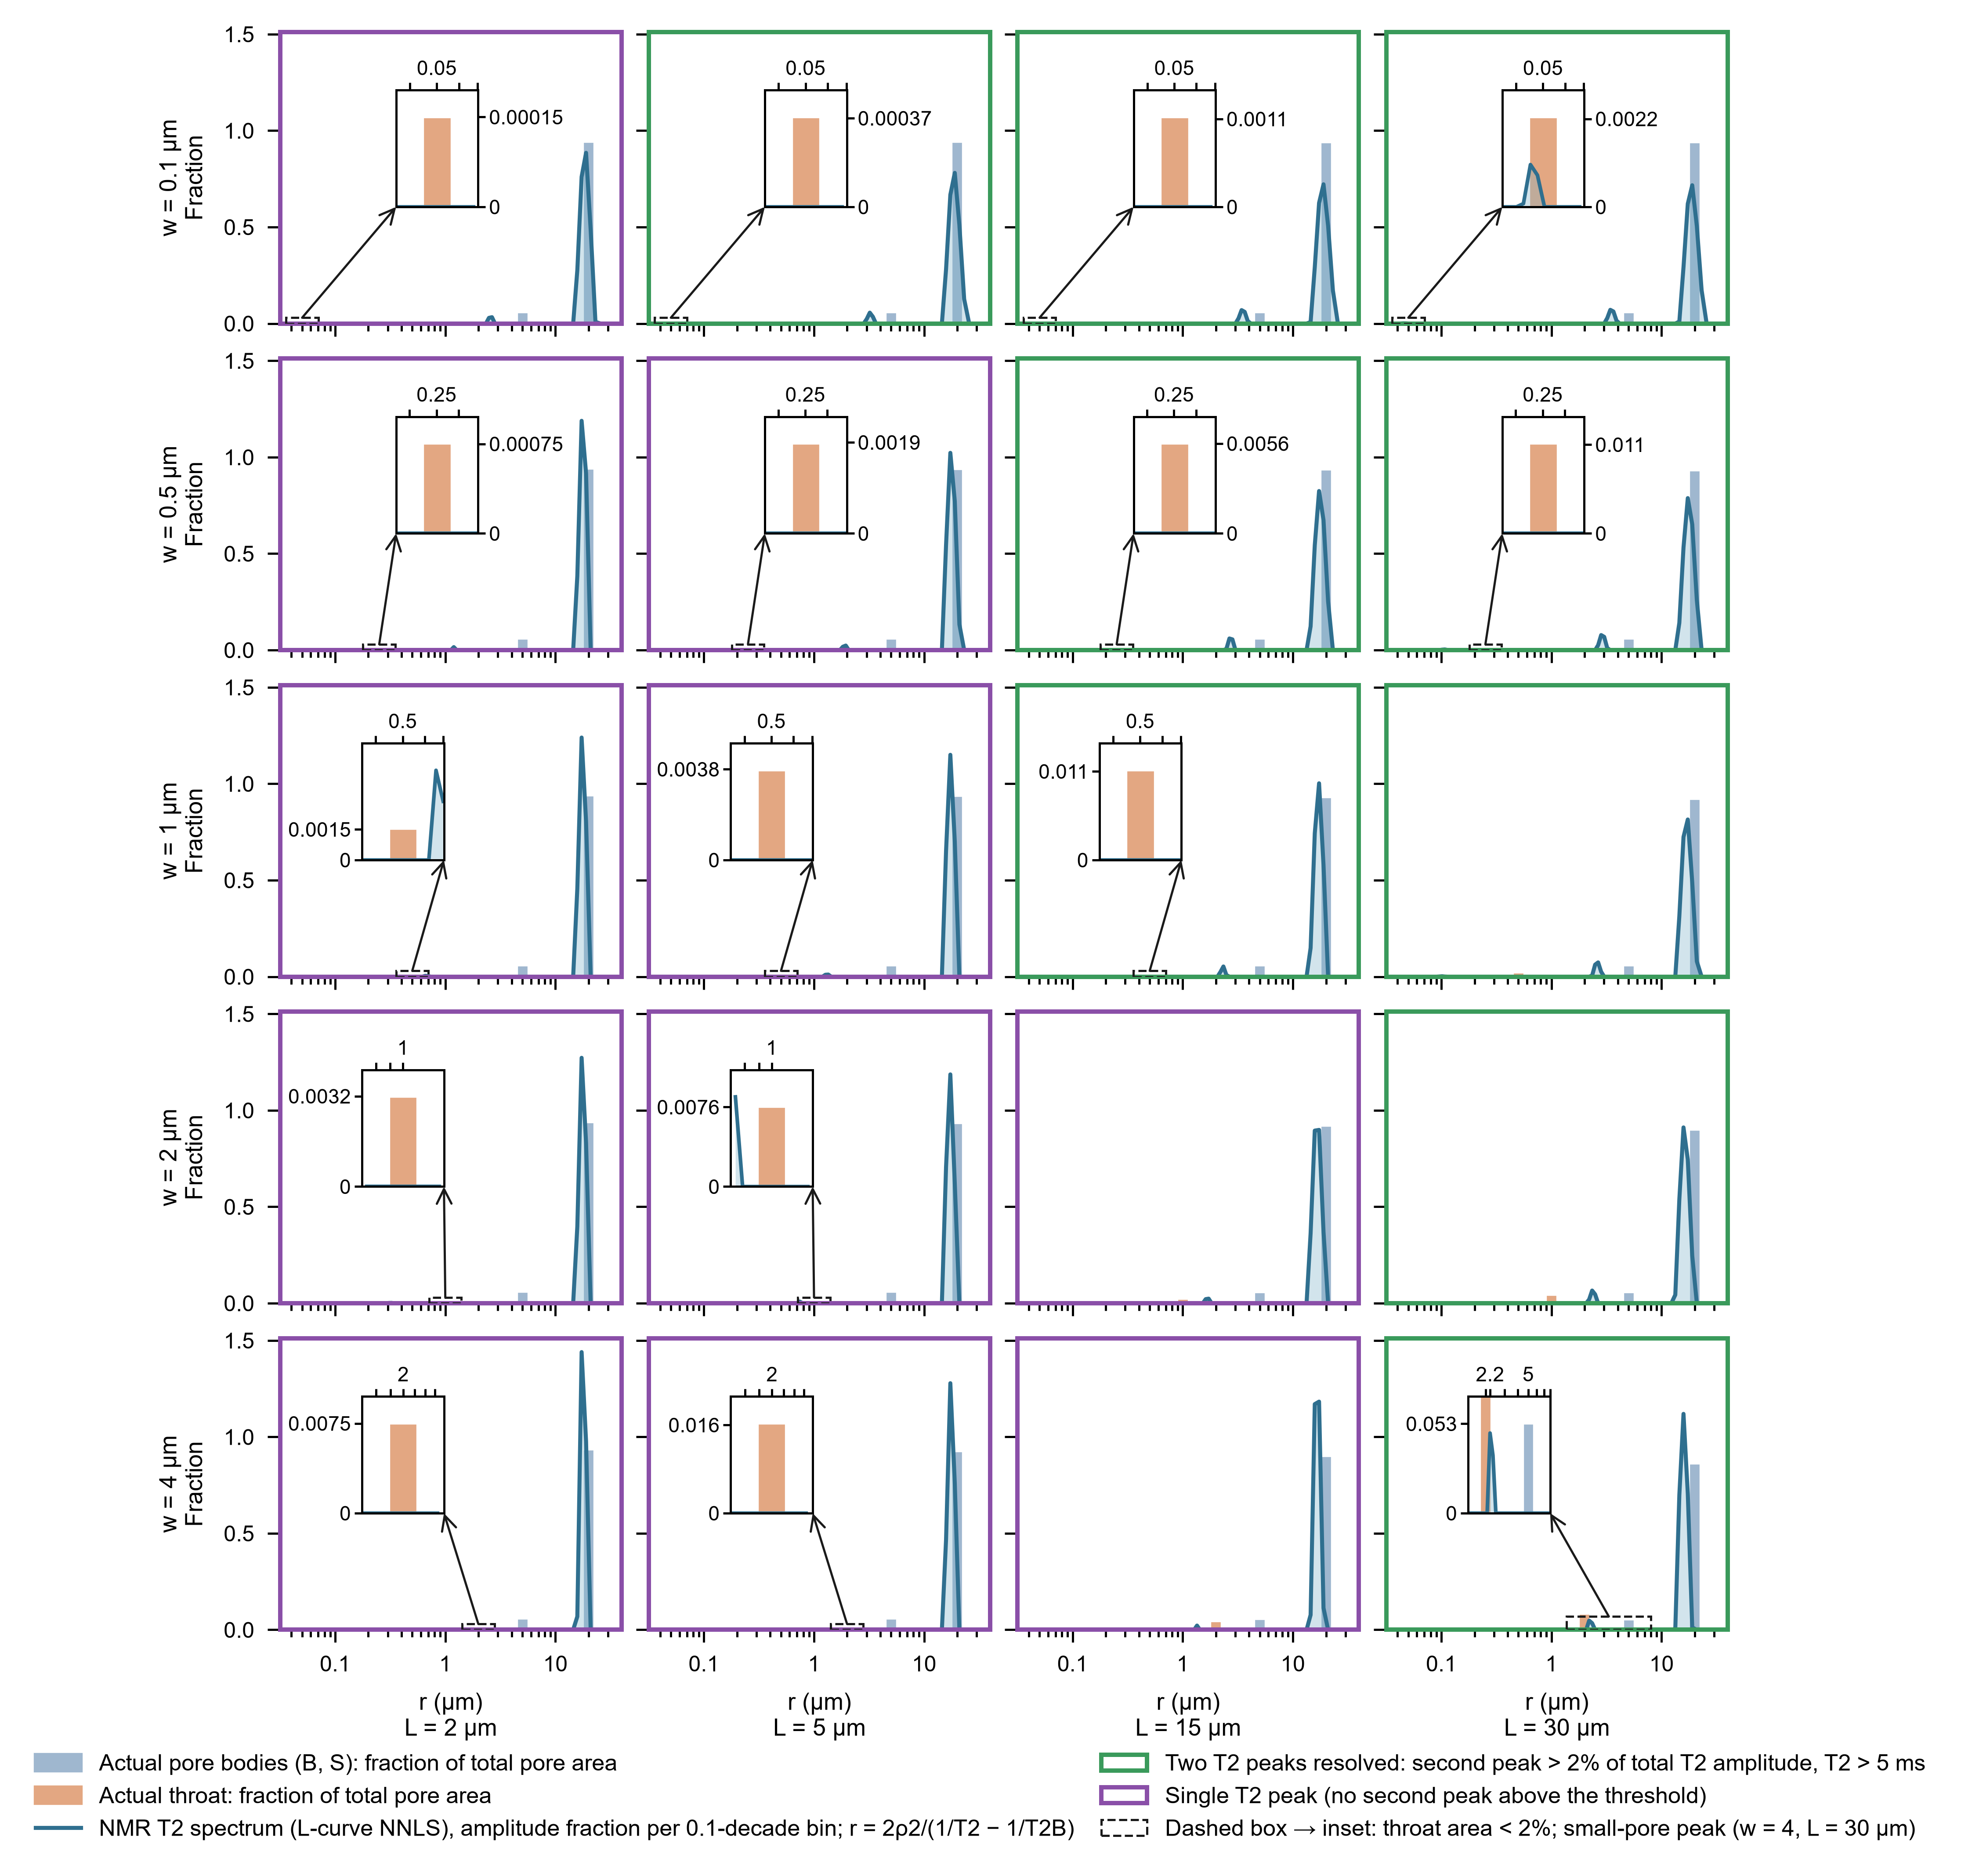
\includegraphics[width=0.92\textwidth]{sweep_overlay_grid.png}
\caption{基准：20 个算例的实际孔体/喉道面积分数直方图与 NNLS（L-curve，SNR 1000）$T_2$ 谱（按 $r=2\rho_2/(1/T_2-1/\TB)$ 映射到半径轴）。
行为喉宽 $w$，列为喉长 $L$。}
\label{fig:baseline}
\end{figure}

\section{模型、参数与数值基准}

几何为闭合单喉道体系：大圆孔 B（$R_B=\SI{20}{\micro m}$）、小圆孔 S（$R_S=\SI{5}{\micro m}$）、一条宽 $w$、壁到壁长 $L$ 的直喉道；
全部固壁以同一 $\rho_2$ 弛豫。数值解为 pyGIMLi 三角网格上的 Bloch–Torrey 隐式 Euler 有限元（$\Delta t=\SI{0.25}{ms}$），
反演为 \texttt{nmr\_t2} 的 NNLS + L-curve\citep{LawsonHanson1974,Hansen1992}。

\begin{table}[H]
\centering\small
\caption{参数与算例（参数与 \texttt{Auto\_NMR.py} 默认值一致，\citealp{Zhou2025}）}
\begin{tabular}{llll}
\toprule
符号 & 含义 & 取值 & 计算单位 \\
\midrule
$D$ & 水的自扩散系数 & \SI{2.0e-9}{m^2/s} & \SI{2.0}{\micro m^2/ms} \\
$\rho_2$ & 表面弛豫率（所有固壁） & \SI{5}{\micro m/s} & \SI{0.005}{\micro m/ms} \\
$\TB$ & 体弛豫时间 & \SI{3}{s} & \SI{3000}{ms} \\
$R_B$, $R_S$ & 大孔、小孔半径 & \SI{20}{\micro m}, \SI{5}{\micro m} & 面积比 $p_S=A_S/(A_S+A_B)=0.0588$ \\
$w$ & 喉宽（半宽 $h=w/2$） & 0.1, 0.5, 1, 2, \SI{4}{\micro m} & \\
$L$ & 喉长（壁到壁） & 2, 5, 15, \SI{30}{\micro m} & 共 $5\times4=20$ 个算例 \\
NNLS & 反演设置 & 200 个对数分箱 $1$--$10^5$ ms & L-curve：$\alpha^2\eta/\zeta\to0.25$；SNR $=1000$ \\
\bottomrule
\end{tabular}
\end{table}

\section{控制方程与孔–喉–孔一维耦合模型}

\subsection{控制方程}
横向磁化满足 Bloch–Torrey 方程与 Robin 表面弛豫边界\citep{Torrey1956,BrownsteinTarr1979}：
\begin{equation}
\frac{\partial M}{\partial t}=D\nabla^2M-\frac{M}{\TB},\qquad D\,\bm n\cdot\nabla M+\rho_2M=0 .
\end{equation}

\subsection{孔体节点与一维喉道}
两孔均处于快扩散区（$\kappa=\rho_2R/D\le0.05$，见前一份解析解文档），孔内磁化浓度可视为均匀 $c_i(t)$，$i\in\{S,B\}$。
孔 $i$ 的面积 $A_i=\pi R_i^2$，弛豫孔壁长度扣除喉口弧长 $P_i=2\pi R_i-2R_i\arcsin(h/R_i)$。对孔体积分得节点方程
\begin{equation}
A_i\frac{\mathrm dc_i}{\mathrm dt}=-R_iA_ic_i-J_i,\qquad R_i=\frac{\rho_2P_i}{A_i}+\frac{1}{\TB},
\label{eq:node}
\end{equation}
$J_i$ 为孔 $i$ 流入喉道的扩散通量。喉道横向扩散时间 $h^2/D$ 远短于 $T_2$，对喉道截面平均得一维扩散–弛豫方程
\begin{equation}
\frac{\partial u}{\partial t}=D\frac{\partial^2u}{\partial x^2}-R_tu,\qquad R_t=\frac{\rho_2}{h}+\frac{1}{\TB},\qquad
u(0,t)=c_S,\quad u(L,t)=c_B,
\label{eq:throat}
\end{equation}
$J_S=-Dw\,\partial_xu|_{x=0}$，$J_B=Dw\,\partial_xu|_{x=L}$。该结构与传热中“肋片–节点”问题相同\citep{CarslawJaeger1959}。

\subsection{本征模与特征方程}
令 $c_i\propto e^{-\lambda t}$、$u=U(x)e^{-\lambda t}$，记 $q^2=(R_t-\lambda)/D$，则
\begin{equation}
U(x)=\frac{c_S\sinh q(L-x)+c_B\sinh qx}{\sinh qL},\qquad
J_S=Dwq\left(c_S\coth qL-c_B\,\mathrm{csch}\,qL\right),
\end{equation}
$J_B$ 同理（$S\leftrightarrow B$）。代入式 \eqref{eq:node}，非零解要求（两边乘以 $S^2$ 消去极点）
\begin{equation}
\boxed{\;\big[(R_S-\lambda)A_S\,S+Dw\,C\big]\big[(R_B-\lambda)A_B\,S+Dw\,C\big]-(Dw)^2=0,\quad S=\frac{\sinh qL}{q},\ C=\cosh qL\;}
\label{eq:char}
\end{equation}
$\lambda>R_t$ 时 $q=\mathrm ik$，$S=\sin kL/k$、$C=\cos kL$（喉道内部模态）。均匀初始磁化下第 $n$ 个模态的信号权重为
\begin{equation}
A_n=\frac{\left(\int_\Omega\phi_n\,\mathrm d\Omega\right)^2}{|\Omega|\int_\Omega\phi_n^2\,\mathrm d\Omega},\qquad
\int_\Omega\phi_n=A_Sc_S+A_Bc_B+w\!\int_0^LU\,\mathrm dx ,
\end{equation}
以下称为 TL（transmission-line）模型。它没有任何拟合参数；对 20 个算例，TL 衰减与全二维有限元衰减的最大偏差
不超过 $|\Delta M/M_0|=0.0065$（图~\ref{fig:valid}a）。

\subsection{准静态约化：带“汇”的两点交换模型}
利用 $\coth x-\mathrm{csch}\,x=\tanh(x/2)$，把喉道通量拆为交换项与汇项：
$J_S=G_x(c_S-c_B)+G_sc_S$，其中
\begin{equation}
G_x=\frac{Dwq}{\sinh qL},\qquad G_s=Dwq\tanh\frac{qL}{2},\qquad q\simeq\sqrt{R_t/D}\quad(\lambda\ll R_t).
\label{eq:gx}
\end{equation}
于是式 \eqref{eq:node} 化为经典两点交换方程\citep{ZimmermanBrittin1957,McDonald2005}
\begin{equation}
\frac{\mathrm d}{\mathrm dt}\begin{pmatrix}m_S\\ m_B\end{pmatrix}=-\begin{pmatrix}R'_S+k_S&-k_B\\-k_S&R'_B+k_B\end{pmatrix}\begin{pmatrix}m_S\\ m_B\end{pmatrix},\qquad
R'_i=R_i+\frac{G_s}{A_i},\quad k_i=\frac{G_x}{A_i},
\end{equation}
$m_i=A_ic_i$，并满足细致平衡 $p_Sk_S=p_Bk_B$。两个极限：
$qL\ll1$ 时 $G_x\to Dw/L$、$G_s\to\tfrac12wLR_t$（喉道体积的弛豫平分给两孔）；
$qL\gg1$ 时 $G_x\to2Dwq\,e^{-qL}\to0$（两孔解耦）、$G_s\to w\sqrt{DR_t}$（半无限喉道成为纯弛豫“汇”）。

\subsection{两点交换的闭式解}
令 $a=R'_S+k_S$，$d=R'_B+k_B$，两个本征速率与快模态权重为
\begin{equation}
\lambda_{f,s}=\frac{a+d\pm\sqrt{(a-d)^2+4k_Sk_B}}{2},
\label{eq:lam}
\end{equation}
\begin{equation}
A_f=\frac{\bar R'-\lambda_s}{\lambda_f-\lambda_s},\qquad \bar R'=p_SR'_S+p_BR'_B,\qquad A_s=1-A_f .
\label{eq:amp}
\end{equation}
式 \eqref{eq:amp} 来自初始斜率：$-\dot s(0)=A_f\lambda_f+A_s\lambda_s=p_SR'_S+p_BR'_B$（交换项因细致平衡相消）。

\subsection{无量纲数与两个极限}
\begin{equation}
\Psi=\frac{Dw/L}{A_S(R_S-R_B)},\qquad
\Peff=\frac{k_S}{R'_S-R'_B},\qquad
\eta=\frac{A_f}{p_S}.
\end{equation}
$\Psi$ 只用几何与孤立孔速率（即原图中的交换数）；$\Peff$ 计入喉道衰减与汇；$\eta$ 为小孔模态保留下来的信号比例。
\begin{itemize}[leftmargin=2em]
\item \textbf{慢交换}（$\Peff\to0$）：$\lambda_f\to R'_S$，$\lambda_s\to R'_B$，$A_f\to p_S$。两个峰分别对应两个孔，权重等于面积分数；
但若 $qL\gtrsim1$，$R'_S=R_S+G_s/A_S$ 中的汇项仍会使小孔峰向短 $T_2$ 偏移，即使两孔之间几乎没有交换。
\item \textbf{快交换}（$\Peff\gg1$）：
\begin{equation}
\lambda_s\to\bar R',\qquad \lambda_f\to\frac{k_S}{p_B},\qquad A_f\approx\frac{p_Sp_B^3}{\Peff^{2}} .
\label{eq:fast}
\end{equation}
主峰位于面积加权的平均速率；快模态仍然存在，但其 $T_2\approx p_BA_S/G_x$ 由交换速率决定（不再反映小孔尺寸），且权重按 $\Peff^{-2}$ 迅速消失。
\end{itemize}

\section{分情况判据}

以 $\eta$ 划分三个区（阈值对应两点交换普适曲线上的 $\Psi\approx0.11$ 与 $\Psi\approx2.0$，$p_S=0.0588$）：
\begin{itemize}[leftmargin=2em]
\item \textbf{区 I，慢交换}（$\eta>0.8$）：两个孔模态，权重近似为面积分数；峰位可能被喉道汇效应偏移。
\item \textbf{区 II，过渡}（$0.1<\eta<0.8$）：小孔峰振幅部分转移到主峰，峰位同时被交换与汇拉向短 $T_2$。
\item \textbf{区 III，快交换}（$\eta<0.1$）：小孔模态仅剩 $A_f<0.1p_S\approx0.6\%$ 的交换模态，主峰位于平均速率；小孔在谱上“消失”。
\end{itemize}
20 个算例中区 I、II、III 分别为 4、8、8 个（表~\ref{tab:regimes}，图~\ref{fig:regime}）。
TL 模型给出的 $\eta$ 和 $T_{2,f}$ 都收敛到两点交换的普适曲线上（图~\ref{fig:regime}b,c）；NNLS 的小峰在区 I、II 与模型一致，
在区 III 则落到噪声与正则化的“底噪”附近（分数 $\le0.5\%$）。
原先以“第二峰面积 $>2\%$”判断单/双峰（图~\ref{fig:oldcontrol}），实际上是在 $\eta\approx0.3$ 附近设了一个探测门槛：
快模态从未真正消失，而是连续地衰减到探测极限以下。

\begin{figure}[H]
\centering
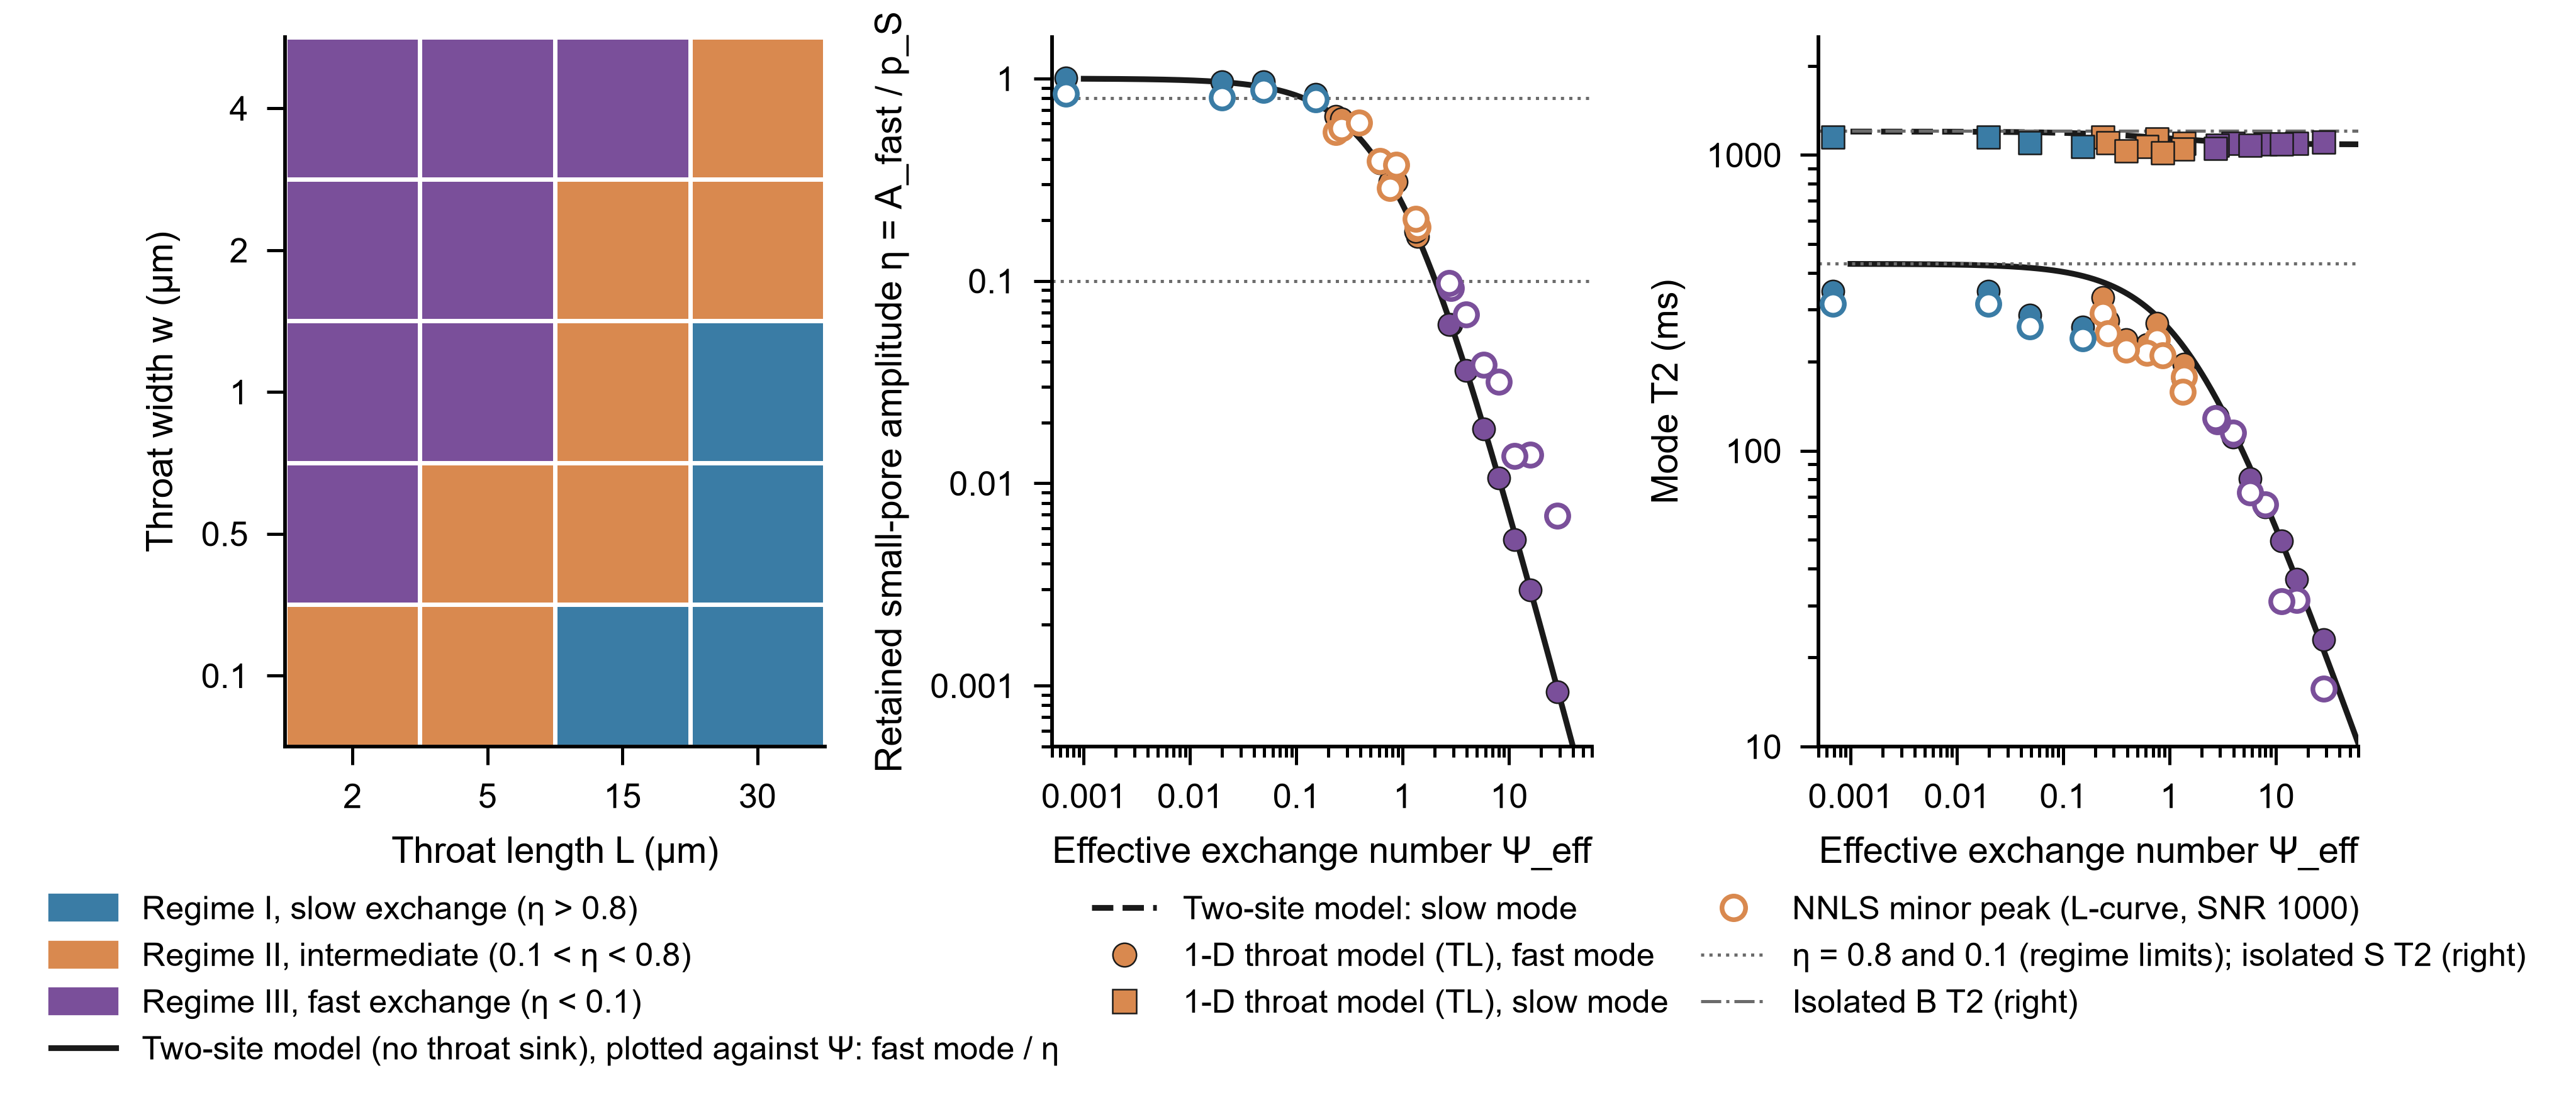
\includegraphics[width=\textwidth]{fig1_regimes_and_universal_curves.png}
\caption{分区与普适曲线。(a) $w$–$L$ 分区图；(b) 小孔模态保留比 $\eta=A_f/p_S$；(c) 模态 $T_2$。黑线为两点交换模型（对 $\Psi$ 作图），
实心点为 TL 模型（对 $\Peff$ 作图），空心点为 NNLS 小峰。}
\label{fig:regime}
\end{figure}

\begin{figure}[H]
\centering
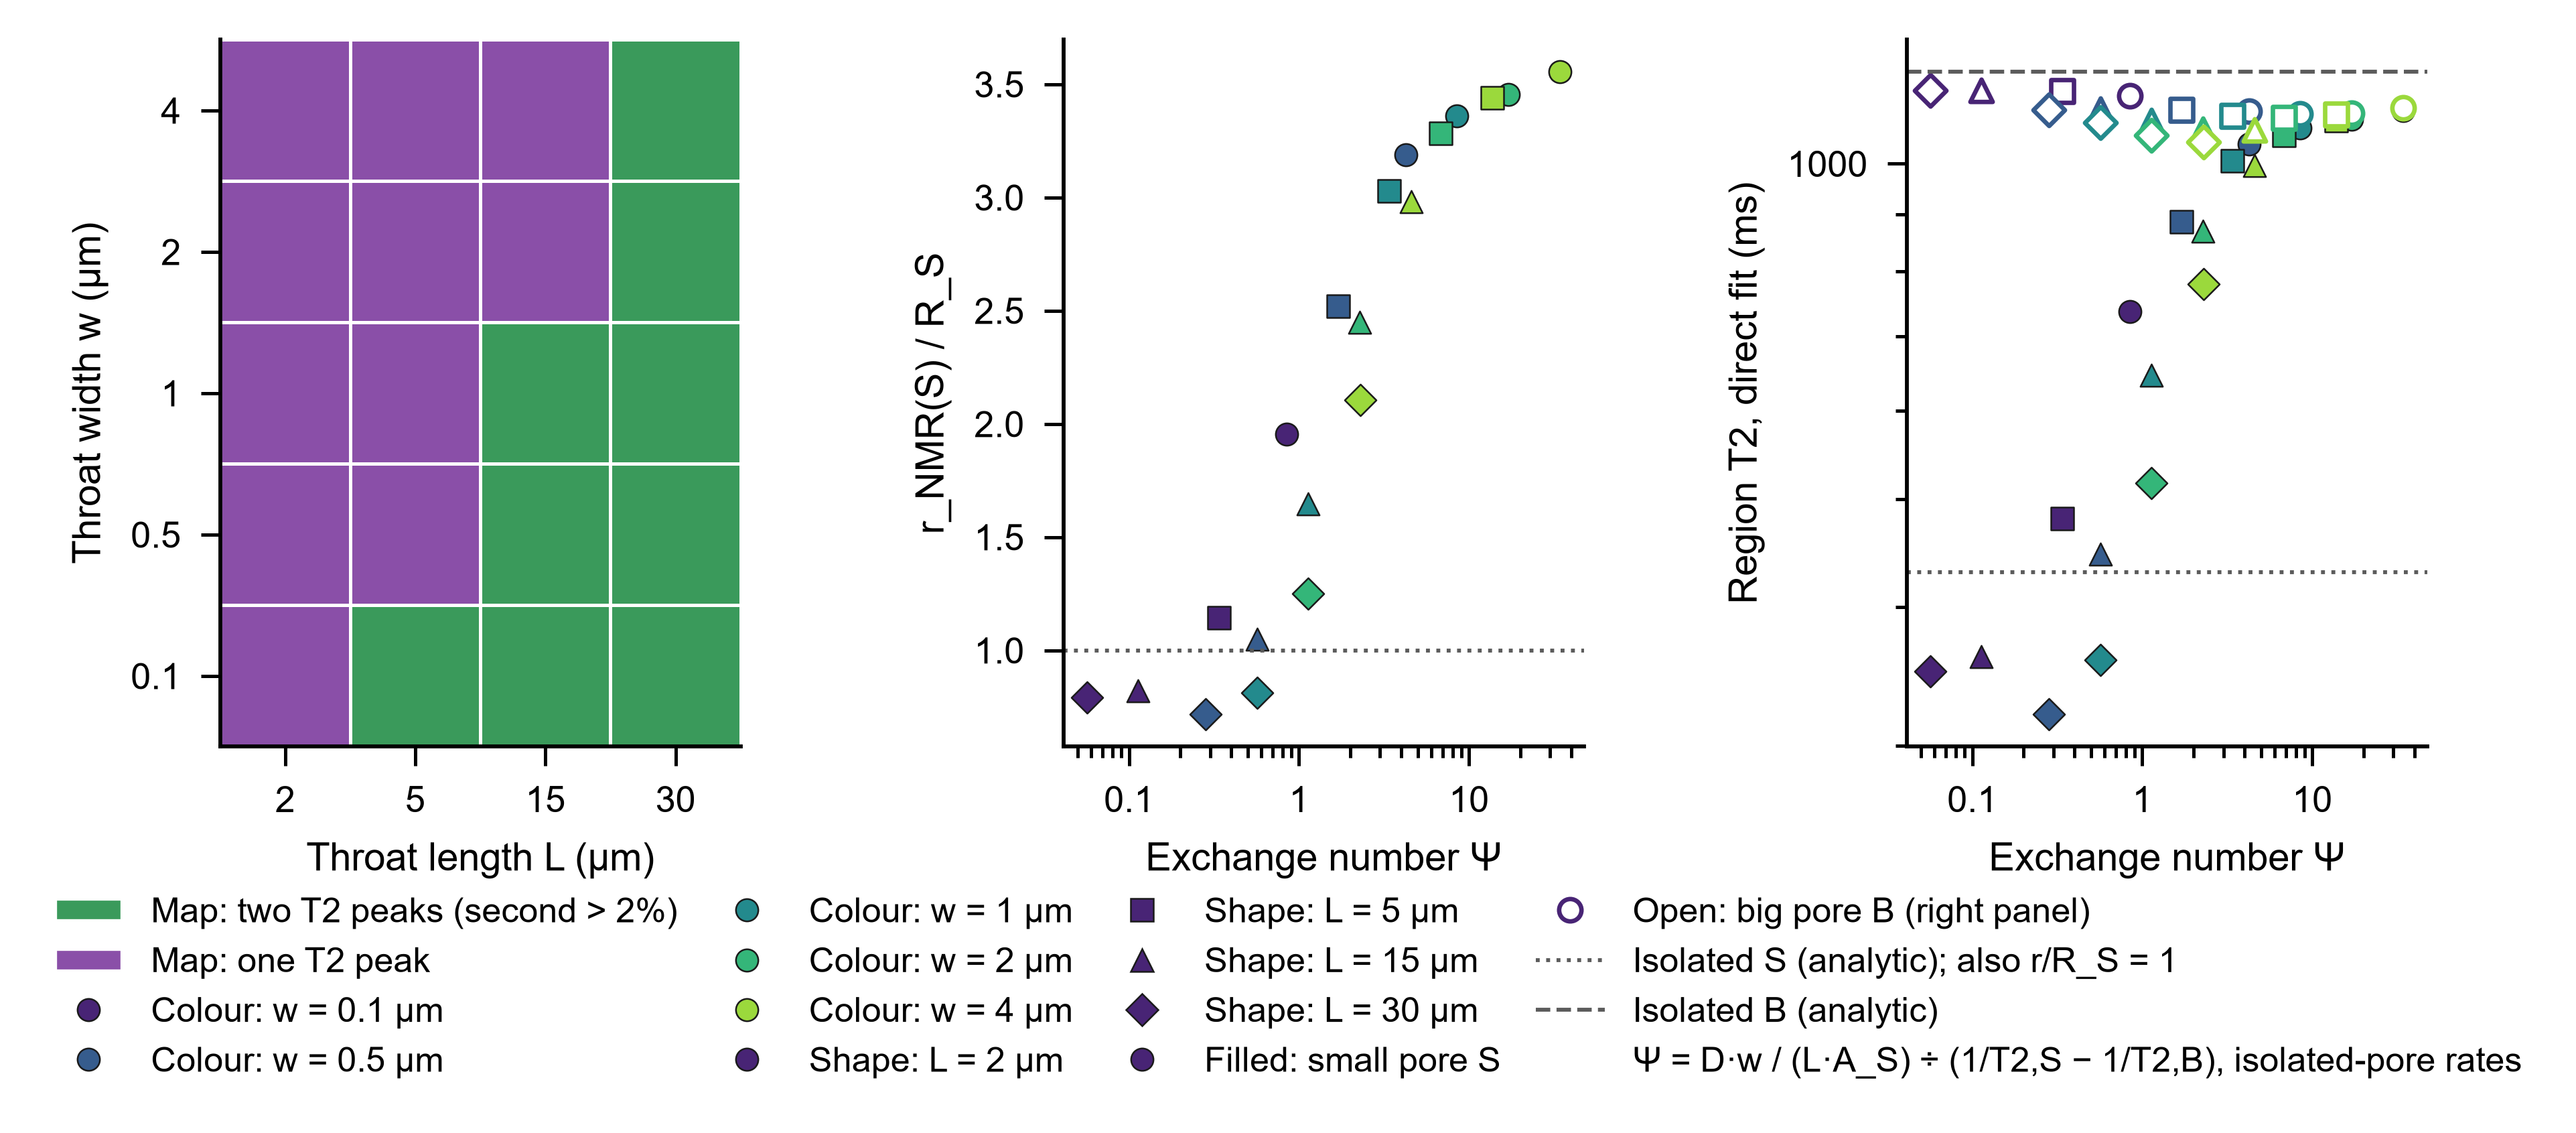
\includegraphics[width=\textwidth]{sweep_coupling_controls.png}
\caption{原耦合控制量图（已重绘图例：每个图例符号都对应图中实际绘制的点；左图改为两类离散色块）。}
\label{fig:oldcontrol}
\end{figure}

\begin{table}[htbp]\centering\small
\caption{20 个算例的无量纲数、分区与小孔模态（TL 模型 vs NNLS，SNR 1000）}\label{tab:regimes}
\begin{tabular}{rrrrrrcrrrr}\toprule
$w$ & $L$ & $\Psi$ & $qL$ & $\Psi_{\mathrm{eff}}$ & $\eta$ & 分区 & \multicolumn{2}{c}{TL：$T_{2,f}$ / $A_f$} & \multicolumn{2}{c}{NNLS：$T_{2\mathrm{lm}}$ / 分数} \\
(\si{\micro m}) & (\si{\micro m}) & & & & & & (ms) & & (ms) & \\ \midrule
0.1 & 2 & 0.852 & 0.448 & 0.764 & 0.310 & II & 269.2 & 0.0182 & 237.2 & 0.0170 \\
0.1 & 5 & 0.341 & 1.12 & 0.236 & 0.651 & II & 329.7 & 0.0383 & 291.7 & 0.0320 \\
0.1 & 15 & 0.114 & 3.36 & 0.0199 & 0.966 & I & 345.9 & 0.0569 & 313.5 & 0.0475 \\
0.1 & 30 & 0.0568 & 6.72 & 0.000679 & 1.005 & I & 346.1 & 0.0591 & 313.8 & 0.0495 \\
0.5 & 2 & 4.31 & 0.202 & 3.96 & 0.036 & III & 111.0 & 0.0021 & 114.9 & 0.0040 \\
0.5 & 5 & 1.73 & 0.505 & 1.38 & 0.165 & II & 196.2 & 0.0097 & 178.1 & 0.0109 \\
0.5 & 15 & 0.577 & 1.51 & 0.265 & 0.632 & II & 275.2 & 0.0372 & 249.5 & 0.0334 \\
0.5 & 30 & 0.289 & 3.03 & 0.0487 & 0.962 & I & 287.3 & 0.0566 & 263.6 & 0.0518 \\
1 & 2 & 8.7 & 0.146 & 7.98 & 0.011 & III & 64.6 & 0.0006 & 65.9 & 0.0019 \\
1 & 5 & 3.51 & 0.362 & 2.83 & 0.061 & III & 131.0 & 0.0036 & 125.5 & 0.0054 \\
1 & 15 & 1.18 & 1.08 & 0.614 & 0.383 & II & 228.8 & 0.0225 & 214.8 & 0.0231 \\
1 & 30 & 0.589 & 2.16 & 0.153 & 0.835 & I & 261.4 & 0.0491 & 239.7 & 0.0466 \\
2 & 2 & 17.4 & 0.11 & 15.8 & 0.003 & III & 36.7 & 0.0002 & 31.4 & 0.0008 \\
2 & 5 & 7.2 & 0.265 & 5.76 & 0.019 & III & 80.6 & 0.0011 & 72.2 & 0.0023 \\
2 & 15 & 2.44 & 0.781 & 1.33 & 0.175 & II & 176.0 & 0.0103 & 158.2 & 0.0119 \\
2 & 30 & 1.23 & 1.56 & 0.389 & 0.596 & II & 237.1 & 0.0351 & 219.7 & 0.0357 \\
4 & 2 & 32.3 & 0.0948 & 28.4 & 0.001 & III & 23.0 & 0.0001 & 15.7 & 0.0004 \\
4 & 5 & 14.7 & 0.208 & 11.3 & 0.005 & III & 49.6 & 0.0003 & 30.9 & 0.0008 \\
4 & 15 & 5.23 & 0.584 & 2.73 & 0.061 & III & 128.6 & 0.0036 & 129.0 & 0.0057 \\
4 & 30 & 2.66 & 1.15 & 0.867 & 0.309 & II & 214.7 & 0.0182 & 210.0 & 0.0221 \\
\bottomrule\end{tabular}\end{table}
\begin{table}[htbp]\centering\footnotesize\setlength{\tabcolsep}{3.5pt}
\caption{代表性算例的代入求解结果：准静态两点交换（手算）、TL 精确根与 NNLS（速率单位 \si{ms^{-1}}，导纳单位 \si{\micro m^2/ms}）}\label{tab:rep}
\resizebox{\textwidth}{!}{%
\begin{tabular}{lrrrrr}\toprule
量 & C1（I） & C2（II） & C3（II） & C4（III） & C5（III） \\ \midrule
$w$, $L$（\si{\micro m}） & 0.1, 30 & 0.5, 15 & 1, 15 & 0.5, 2 & 4, 2 \\
$L_m$（网格壁到壁，\si{\micro m}） & 30.000 & 15.008 & 15.031 & 2.008 & 2.518 \\
$P_S$, $P_B$（\si{\micro m}） & 31.32, 125.56 & 30.92, 125.16 & 30.41, 124.66 & 30.92, 125.16 & 27.30, 121.66 \\
$R_S$ & $2.327\times10^{-3}$ & $2.301\times10^{-3}$ & $2.270\times10^{-3}$ & $2.301\times10^{-3}$ & $2.071\times10^{-3}$ \\
$R_B$ & $8.329\times10^{-4}$ & $8.313\times10^{-4}$ & $8.294\times10^{-4}$ & $8.313\times10^{-4}$ & $8.174\times10^{-4}$ \\
$R_t$ & $0.1003$ & $0.02033$ & $0.01033$ & $0.02033$ & $2.833\times10^{-3}$ \\
$q$（\si{\micro m^{-1}}）, $qL$ & 0.2240, 6.719 & 0.1008, 1.513 & 0.0719, 1.080 & 0.1008, 0.202 & 0.0376, 0.095 \\
$G_x$ & $1.082\times10^{-4}$ & $0.04667$ & $0.1103$ & $0.4947$ & $3.173$ \\
$G_s$ & $0.04469$ & $0.06444$ & $0.07090$ & $0.01017$ & $0.01426$ \\
$R'_S$ & $2.896\times10^{-3}$ & $3.122\times10^{-3}$ & $3.172\times10^{-3}$ & $2.431\times10^{-3}$ & $2.253\times10^{-3}$ \\
$R'_B$ & $8.685\times10^{-4}$ & $8.826\times10^{-4}$ & $8.858\times10^{-4}$ & $8.394\times10^{-4}$ & $8.287\times10^{-4}$ \\
$k_S$ & $1.377\times10^{-6}$ & $5.942\times10^{-4}$ & $1.404\times10^{-3}$ & $6.298\times10^{-3}$ & $0.04040$ \\
$\Psi_{\mathrm{eff}}$ & 0.0006792 & 0.2653 & 0.6143 & 3.957 & 28.37 \\
手算 $T_{2,f}$ / $T_{2,s}$（ms） & 345.1 / 1151.3 & 268.5 / 1096.6 & 216.9 / 1064.2 & 110.5 / 1092.0 & 22.2 / 1098.9 \\
手算 $A_f$ & $0.0587$ & $0.0364$ & $0.0220$ & $0.0021$ & $5.75\times10^{-5}$ \\
TL $T_{2,f}$ / $T_{2,s}$（ms） & 346.1 / 1151.5 & 275.2 / 1098.7 & 228.8 / 1069.7 & 111.0 / 1092.7 & 23.0 / 1107.0 \\
TL $A_f$（$\eta$） & $0.0591$ ($1.0049$) & $0.0372$ ($0.6325$) & $0.0225$ ($0.3827$) & $0.0021$ ($0.0360$) & $5.50\times10^{-5}$ ($9.35\times10^{-4}$) \\
NNLS $T_{2\mathrm{lm}}$：小峰 / 主峰（ms） & 313.8 / 1154.4 & 249.5 / 1109.6 & 214.8 / 1086.7 & 114.9 / 1111.7 & 15.7 / 1121.1 \\
NNLS 小峰分数 & 0.0495 & 0.0334 & 0.0231 & 0.0040 & 0.0004 \\
TL 衰减最大误差 $|\Delta M/M_0|$ & 0.0036 & 0.0047 & 0.0055 & 0.0058 & 0.0046 \\
\bottomrule\end{tabular}}\end{table}
\begin{table}[htbp]\centering\footnotesize\setlength{\tabcolsep}{4pt}
\caption{代表性算例的反算孔径（\si{\micro m}，SNR 1000；真值 $r_S=5$、$r_B=20$）}\label{tab:back}
\begin{tabular}{lcccccc}\toprule
算例 & 分区 & 路线 A & 路线 B & 路线 C & 路线 D & 路线 D（精确模态） \\
 & & $r_S$ / $r_B$ & $r_S$ / $r_B$ & $r_S$ / $r_B$ & $r_S$ / $r_B$ & $r_S$ / $r_B$ \\ \midrule
C1（$w$=0.1, $L$=30） & I & 3.50 / 18.76 & 4.28 / 18.76 & 3.73 / 16.59 & 4.57 / 20.09 & 5.00 / 19.99 \\
C2（$w$=0.5, $L$=15） & II & 2.72 / 17.61 & 3.27 / 17.61 & 2.88 / 15.72 & 4.65 / 19.88 & 5.00 / 20.00 \\
C3（$w$=1, $L$=15） & II & 2.31 / 17.04 & 2.62 / 17.04 & 2.40 / 15.78 & 4.84 / 19.61 & 5.00 / 20.00 \\
C4（$w$=0.5, $L$=2） & III & 1.19 / 17.66 & 1.12 / 17.66 & 1.72 / 18.15 & 5.50 / 17.98 & 5.00 / 20.00 \\
C5（$w$=4, $L$=2） & III & 0.16 / 17.90 & 0.36 / 17.90 & 0.17 / 15.21 & 16.10 / 5.56 & 5.00 / 20.00 \\
\bottomrule\end{tabular}\end{table}
\begin{table}[htbp]\centering\small
\caption{同一算例在 SNR 100 下的 NNLS 小峰与反算（\si{\micro m}）}\label{tab:snr}
\begin{tabular}{lcccccc}\toprule
算例 & 小峰 $T_{2\mathrm{lm}}$ (ms) & 小峰分数 & A：$r_S$ & B：$r_S$ & D：$r_S$ / $r_B$ & 主峰按 A：$r_B$ \\ \midrule
C1 & 142.8 & 0.0183 & 1.50 & 2.44 & 2.39 / 18.26 & 17.87 \\
C2 & 100.5 & 0.0137 & 1.04 & 2.01 & 2.41 / 17.20 & 17.02 \\
C3 & 58.4 & 0.0086 & 0.60 & 1.55 & 1.90 / 15.16 & 16.56 \\
C4 & 无 & 0 & -- & -- & -- & 17.45 \\
C5 & 无 & 0 & -- & -- & -- & 17.74 \\
\bottomrule\end{tabular}\end{table}


\begin{figure}[H]
\centering
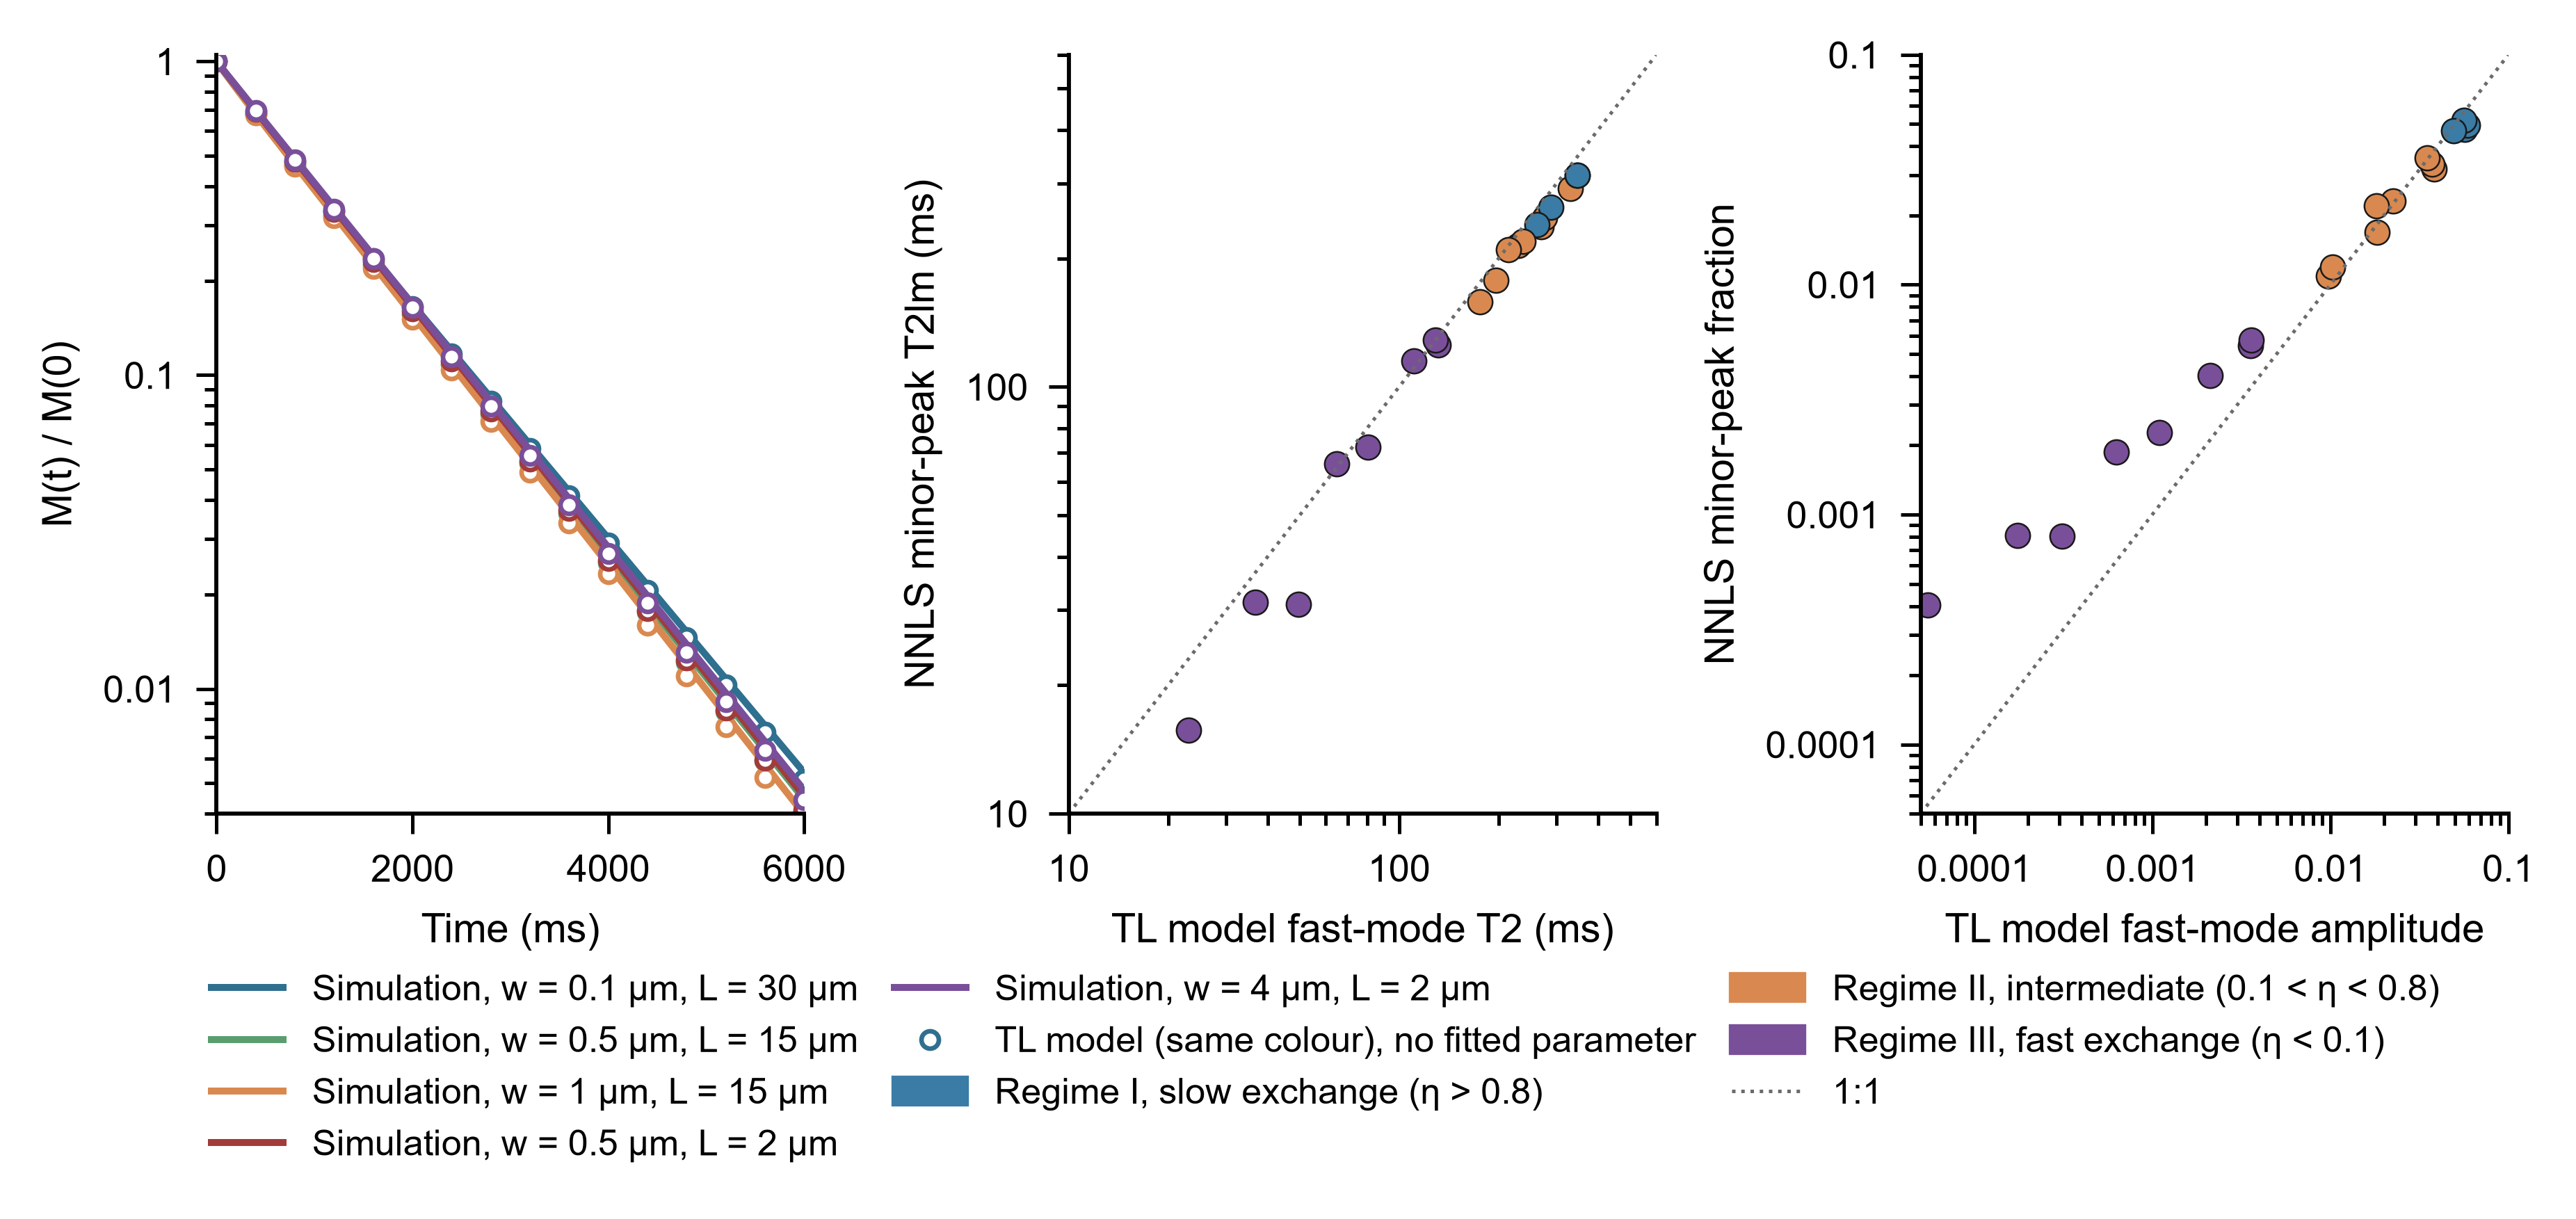
\includegraphics[width=\textwidth]{fig2_model_validation.png}
\caption{模型验证。(a) 5 个代表算例的全二维模拟衰减（实线）与 TL 模型（空心点，无拟合参数）；(b,c) TL 快模态 $T_2$ 与权重对 NNLS 小峰。}
\label{fig:valid}
\end{figure}

\section{代表性算例的代入求解}

代表算例：C1（$w=0.1$，$L=30$，区 I）、C2（$0.5$，$15$，区 II）、C3（$1$，$15$，区 II）、C4（$0.5$，$2$，区 III）、C5（$4$，$2$，区 III），单位 \si{\micro m}。
全部数值见表~\ref{tab:rep}；下面逐步给出 C3 的代入过程与 C5 的快交换渐近式。

\subsection{算例 C3（$w=\SI{1}{\micro m}$，$L=\SI{15}{\micro m}$，区 II）的逐步代入}
\textbf{第 1 步：几何与孔体速率。}网格中喉道壁到壁长度 $L_m=15.031$~\si{\micro m}，喉口弧长 $2R\arcsin(h/R)$ 从孔壁中扣除：
\begin{align*}
A_S&=\pi\times5^2=78.540, & P_S&=2\pi\times5-1.0017=30.414,\\
A_B&=\pi\times20^2=1256.64, & P_B&=2\pi\times20-1.0001=124.664,\\
R_S&=\frac{0.005\times30.414}{78.540}+\frac{1}{3000}=2.270\times10^{-3}\ \mathrm{ms^{-1}}, & R_B&=8.294\times10^{-4}\ \mathrm{ms^{-1}}.
\end{align*}
\textbf{第 2 步：喉道。}$h=\SI{0.5}{\micro m}$：
\[
R_t=\frac{0.005}{0.5}+\frac{1}{3000}=0.01033,\qquad q=\sqrt{R_t/D}=\sqrt{0.01033/2.0}=0.07188\ \mathrm{\mu m^{-1}},\qquad qL=1.0804.
\]
\textbf{第 3 步：交换导纳与汇导纳（式 \eqref{eq:gx}）。}
\[
G_x=\frac{Dwq}{\sinh qL}=\frac{2.0\times1\times0.07188}{\sinh 1.0804}=0.1103,\qquad
G_s=Dwq\tanh\frac{qL}{2}=0.07090\ \mathrm{\mu m^2/ms}.
\]
\textbf{第 4 步：有效两点交换参数。}
\begin{align*}
R'_S&=R_S+\frac{G_s}{A_S}=2.270\times10^{-3}+9.027\times10^{-4}=3.172\times10^{-3}, & R'_B&=8.858\times10^{-4},\\
k_S&=\frac{G_x}{A_S}=1.404\times10^{-3}, & k_B&=\frac{G_x}{A_B}=8.778\times10^{-5},\\
\Psi_{\mathrm{eff}}&=\frac{k_S}{R'_S-R'_B}=\frac{1.404\times10^{-3}}{2.286\times10^{-3}}=0.6143. &&
\end{align*}
\textbf{第 5 步：本征速率（式 \eqref{eq:lam}）。}$a=R'_S+k_S=4.577\times10^{-3}$，$d=R'_B+k_B=9.736\times10^{-4}$：
\begin{align*}
\lambda_{f,s}&=\frac{a+d\pm\sqrt{(a-d)^2+4k_Sk_B}}{2}=\frac{5.550\times10^{-3}\pm3.671\times10^{-3}}{2}\\
&\Rightarrow\;T_{2,f}=1/\lambda_f=216.9\ \mathrm{ms},\qquad T_{2,s}=1/\lambda_s=1064.2\ \mathrm{ms}.
\end{align*}
\textbf{第 6 步：快模态振幅（式 \eqref{eq:amp}）。}
\[
\bar R'=p_SR'_S+p_BR'_B=1.020\times10^{-3},\qquad A_f=\frac{\bar R'-\lambda_s}{\lambda_f-\lambda_s}=0.0220,\qquad \eta=\frac{A_f}{p_S}=0.373.
\]
\textbf{第 7 步：对照。}TL 精确根给出 $T_{2,f}=228.8$~ms、$A_f=0.0225$；
NNLS（L-curve，SNR 1000）小峰 $T_{2\mathrm{lm}}=214.8$~ms、分数 0.0231；手算与精确根的差别来自准静态近似中 $q$ 取 $\lambda=0$。

\subsection{快交换算例 C5（$w=\SI{4}{\micro m}$，$L=\SI{2}{\micro m}$，区 III）的渐近式}
\[
\Psi_{\mathrm{eff}}=28.37,\qquad A_f\approx\frac{p_Sp_B^3}{\Psi_{\mathrm{eff}}^2}=\frac{0.0588\times0.9412^3}{28.37^2}=6.09\times10^{-5}\quad(\text{TL 精确}\ 5.50\times10^{-5}),
\]
\[
T_{2,f}\approx\frac{p_BA_S}{G_x}=\frac{0.9412\times78.54}{3.1728}=23.3\ \mathrm{ms}\quad(\text{TL}\ 23.0\ \mathrm{ms},\ \text{NNLS}\ 15.7\ \mathrm{ms}).
\]
快模态的 $T_2$ 由交换速率决定，而不是由小孔的 $S/V$ 决定；若按孤立孔公式换算，会得到一个并不存在的 0.16~\si{\micro m} 的“孔”。

\subsection{反算的代入示例}
\textbf{路线 A（C3）：}
\[
r_S=\frac{2\rho_2}{1/T_{2,f}-1/T_{2B}}=\frac{0.01}{1/214.79-1/3000}=2.31\ \mu\mathrm{m},\qquad r_B=\frac{0.01}{1/1086.72-1/3000}=17.04\ \mu\mathrm{m}.
\]
\textbf{路线 B（C1）：}小峰分数 $f_S=0.0495$，主峰按路线 A 得 $r_B=18.76$~\si{\micro m}：
\[
r_S=r_B\sqrt{\frac{f_S}{1-f_S}}=18.76\times\sqrt{\frac{0.0495}{0.9505}}=4.28\ \mu\mathrm{m}.
\]
\textbf{区 III 的有效半径（C5）：}主峰 $T_{2\mathrm{lm}}=1121.08$~ms，
\[
R_{\mathrm{eff}}=\frac{0.01}{1/1121.08-1/3000}=17.90\ \mu\mathrm{m}\quad\text{vs.}\quad\frac{r_B^2+r_S^2}{r_B+r_S}=\frac{400+25}{25}=17.00\ \mu\mathrm{m}.
\]


\section{反算方法与结果}

\subsection{四条反算路线}
\begin{description}[leftmargin=2em,style=nextline]
\item[路线 A：孤立孔公式]
对每个 NNLS 峰的 $T_{2\mathrm{lm}}$ 用 $r=2\rho_2/(1/T_2-1/\TB)$。只在两孔完全解耦且无喉道汇时成立。
\item[路线 B：振幅比]
二维圆孔的面积分数 $p_S=r_S^2/(r_S^2+r_B^2)$，区 I 中 $A_f\approx p_S$，故
\begin{equation}
r_S=r_B\sqrt{f_S/f_B},
\end{equation}
$r_B$ 取主峰按路线 A 的值。振幅反映的是体积（面积）分数，对汇效应不敏感。
\item[路线 C：两点交换反演（不知喉道）]
未知 $(r_S,r_B,G)$，用 $(\lambda_f,\lambda_s,A_f)$ 三个观测量求解式 \eqref{eq:lam}–\eqref{eq:amp}（不含汇）。
\item[路线 D：TL 模型反演（喉道已知）]
已知 $w$、$L$（如来自成像或 SIP 的喉道信息），未知 $(r_S,r_B)$，以 $\ln\lambda_f$、$\ln\lambda_s$、$\ln A_f$ 的残差最小二乘求解式 \eqref{eq:char}。
\end{description}

\subsection{结果}
结果见表~\ref{tab:back} 与图~\ref{fig:back}：
\begin{itemize}[leftmargin=2em]
\item 路线 A 在所有耦合算例中低估小孔（区 I 为 3.5~\si{\micro m}，区 III 为把交换模态误读成 0.16–1.2~\si{\micro m} 的“伪孔”），主孔低估 6–15\%。
\item 路线 B 在区 I 将小孔改善到 4.3~\si{\micro m}，但在区 II、III 因 $A_f<p_S$ 而失效。
\item 路线 C 收敛到 $G\to0$ 且残差不为零：在存在喉道汇时，三个观测量与任何“无汇两点交换 + 真实孔径”都不自洽，不知道喉道就无法区分交换与汇。
\item 路线 D 在区 I、II 恢复 $r_S=4.6$–$4.8$、$r_B=19.6$–$20.1$~\si{\micro m}；以精确模态作输入时五个算例均恢复 $5.00/20.0$~\si{\micro m}，
说明剩余误差来自 NNLS 正则化偏差而非模型。区 III 中 C4 的 0.4\% 交换模态仍给出近似值（$5.5/18.0$，误差约 10\%），C5 的 0.04\% 已在噪声中，反算失败。
\end{itemize}

\begin{figure}[H]
\centering
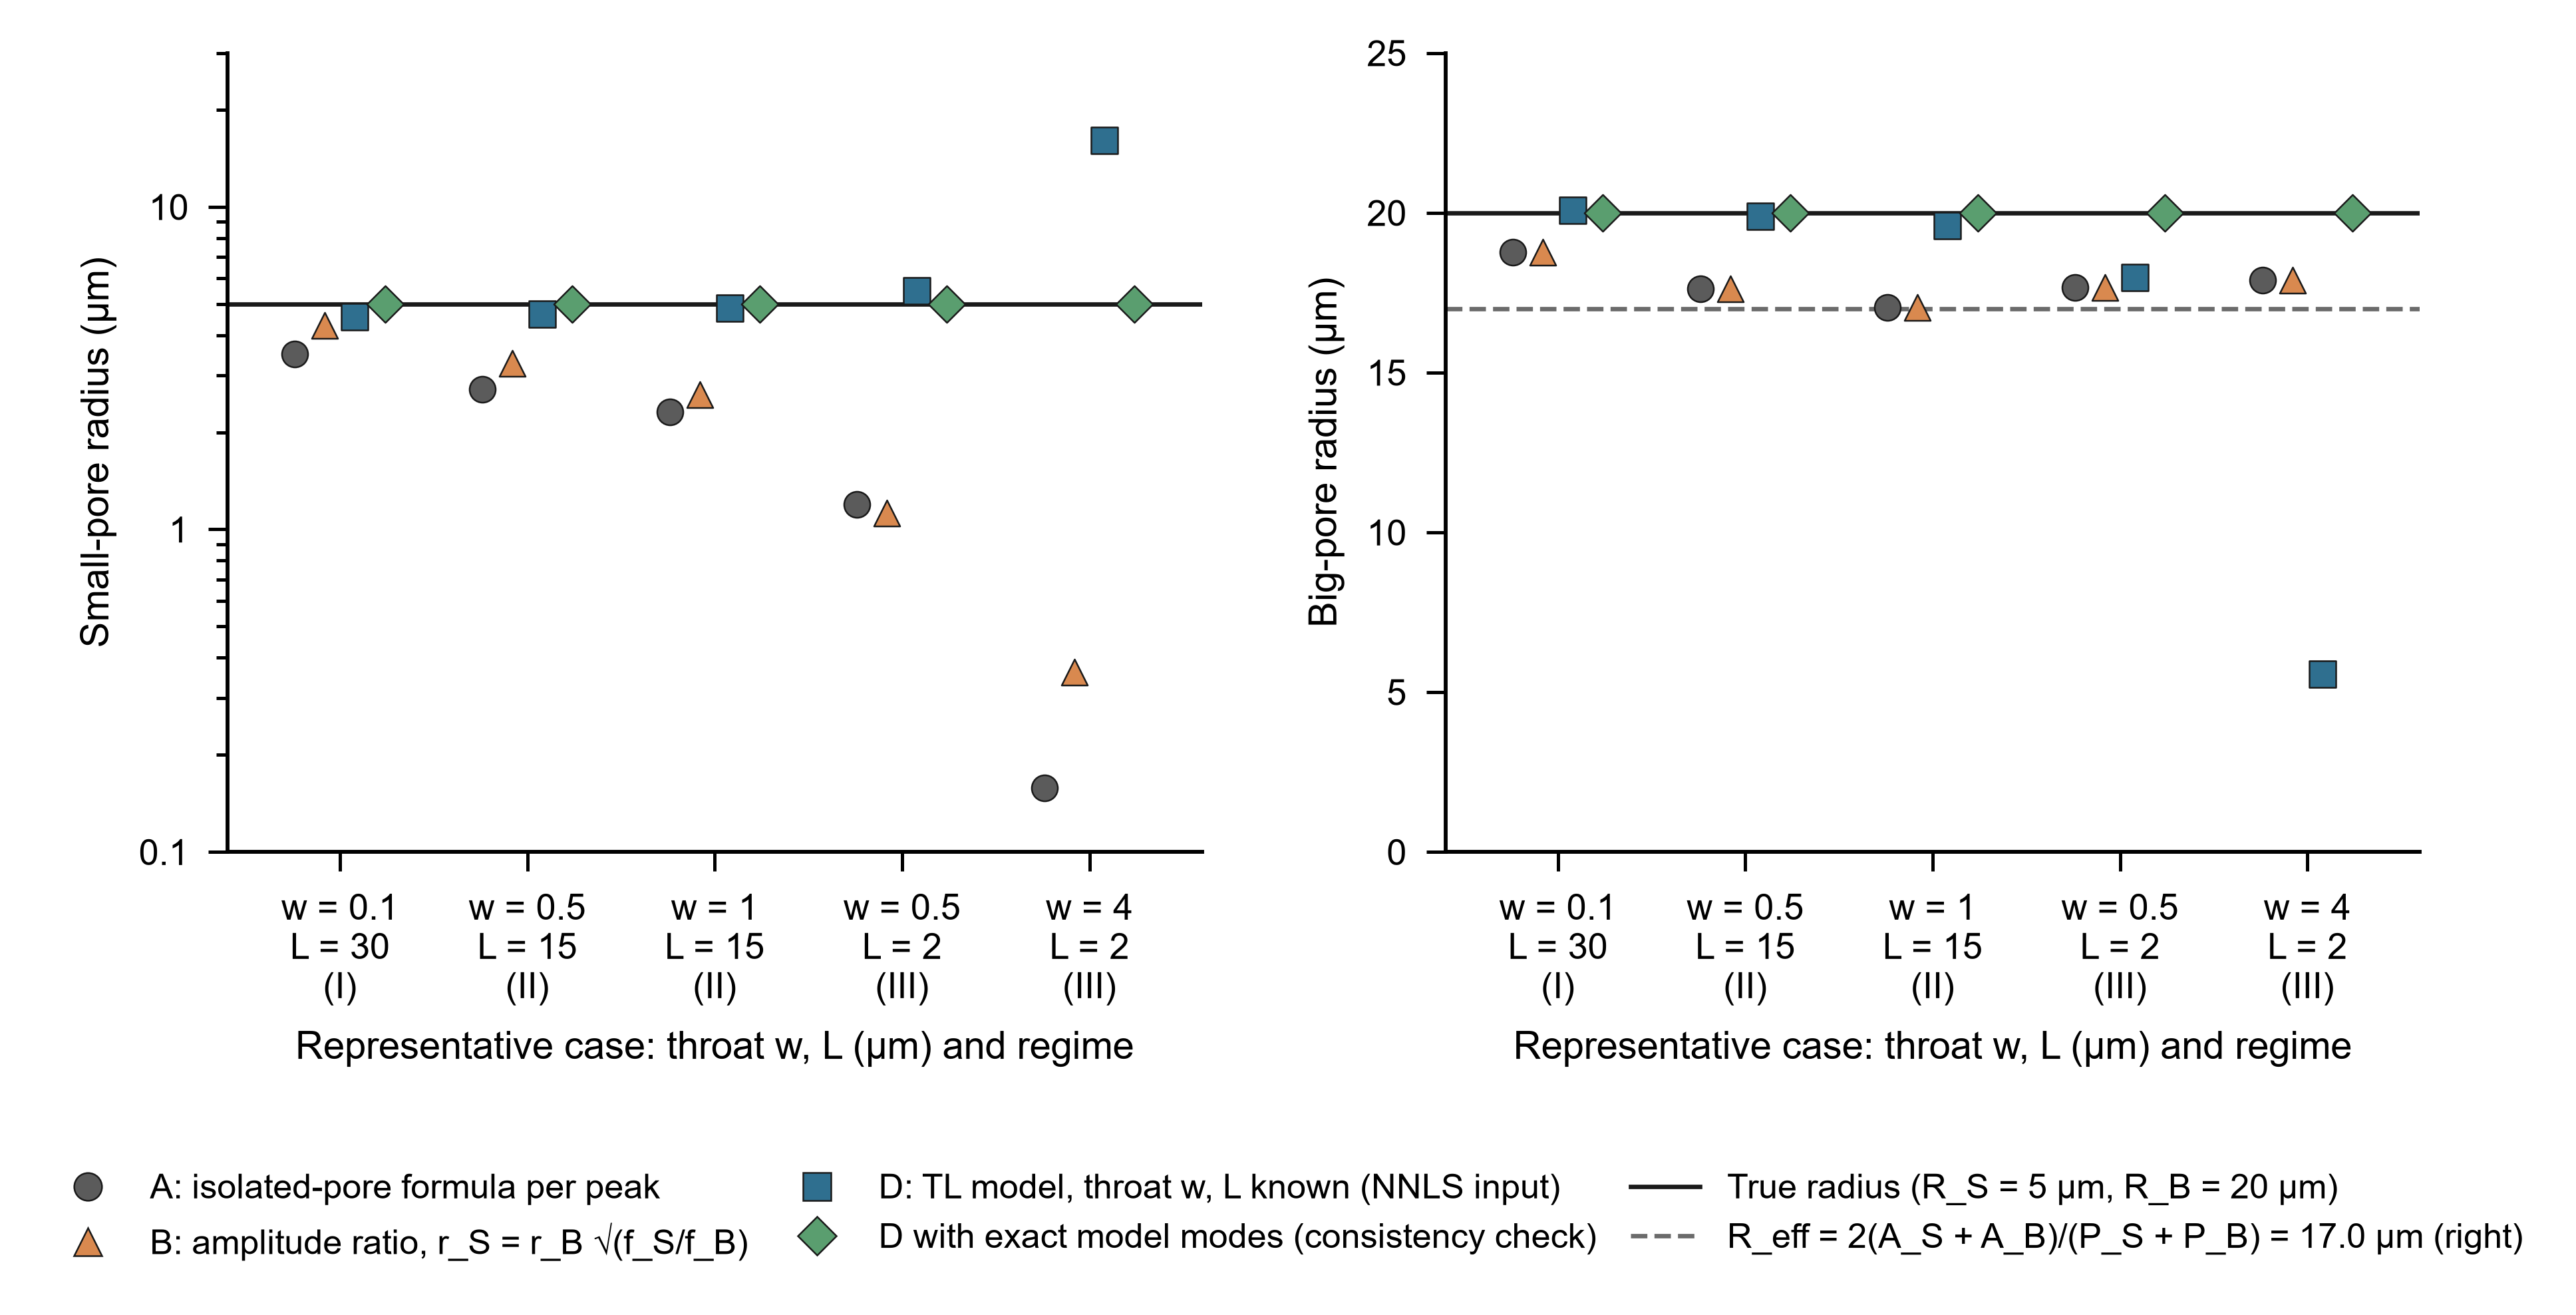
\includegraphics[width=\textwidth]{fig3_backcalculated_sizes.png}
\caption{代表算例的反算孔径（SNR 1000）。左：小孔；右：大孔（虚线为区 III 唯一可确定的 $R_{\mathrm{eff}}$）。}
\label{fig:back}
\end{figure}

\subsection{为什么小孔会被“忽略”}
区 III 中主峰速率 $\lambda_s\to\bar R$，按孤立孔公式换算得到的是两孔合并后的等效半径
\begin{equation}
R_{\mathrm{eff}}=\frac{2\rho_2}{\bar R-1/\TB}=\frac{2(A_S+A_B)}{P_S+P_B}=\frac{r_B^2+r_S^2}{r_B+r_S}\quad(\text{二维圆孔}),
\label{eq:reff}
\end{equation}
本例为 17.0~\si{\micro m}，NNLS 主峰给出 17.7–17.9~\si{\micro m}。式 \eqref{eq:reff} 是一条曲线而不是一个点（图~\ref{fig:nonunique}）：
任何满足它的 $(r_S,r_B)$ 都给出几乎相同的单峰谱，因此单靠 $T_2$ 无法分离两种孔，按“单一孔隙”解读就等于把小孔忽略、并把主孔低估约 11\%。
要恢复小孔需要额外约束：喉道几何（路线 D，须足够高的 SNR 以保留交换模态）、孔隙体积分配（CT）、或 $T_2$–$T_2$ 交换谱\citep{McDonald2005,FleurySoualem2009}。

\begin{figure}[H]
\centering
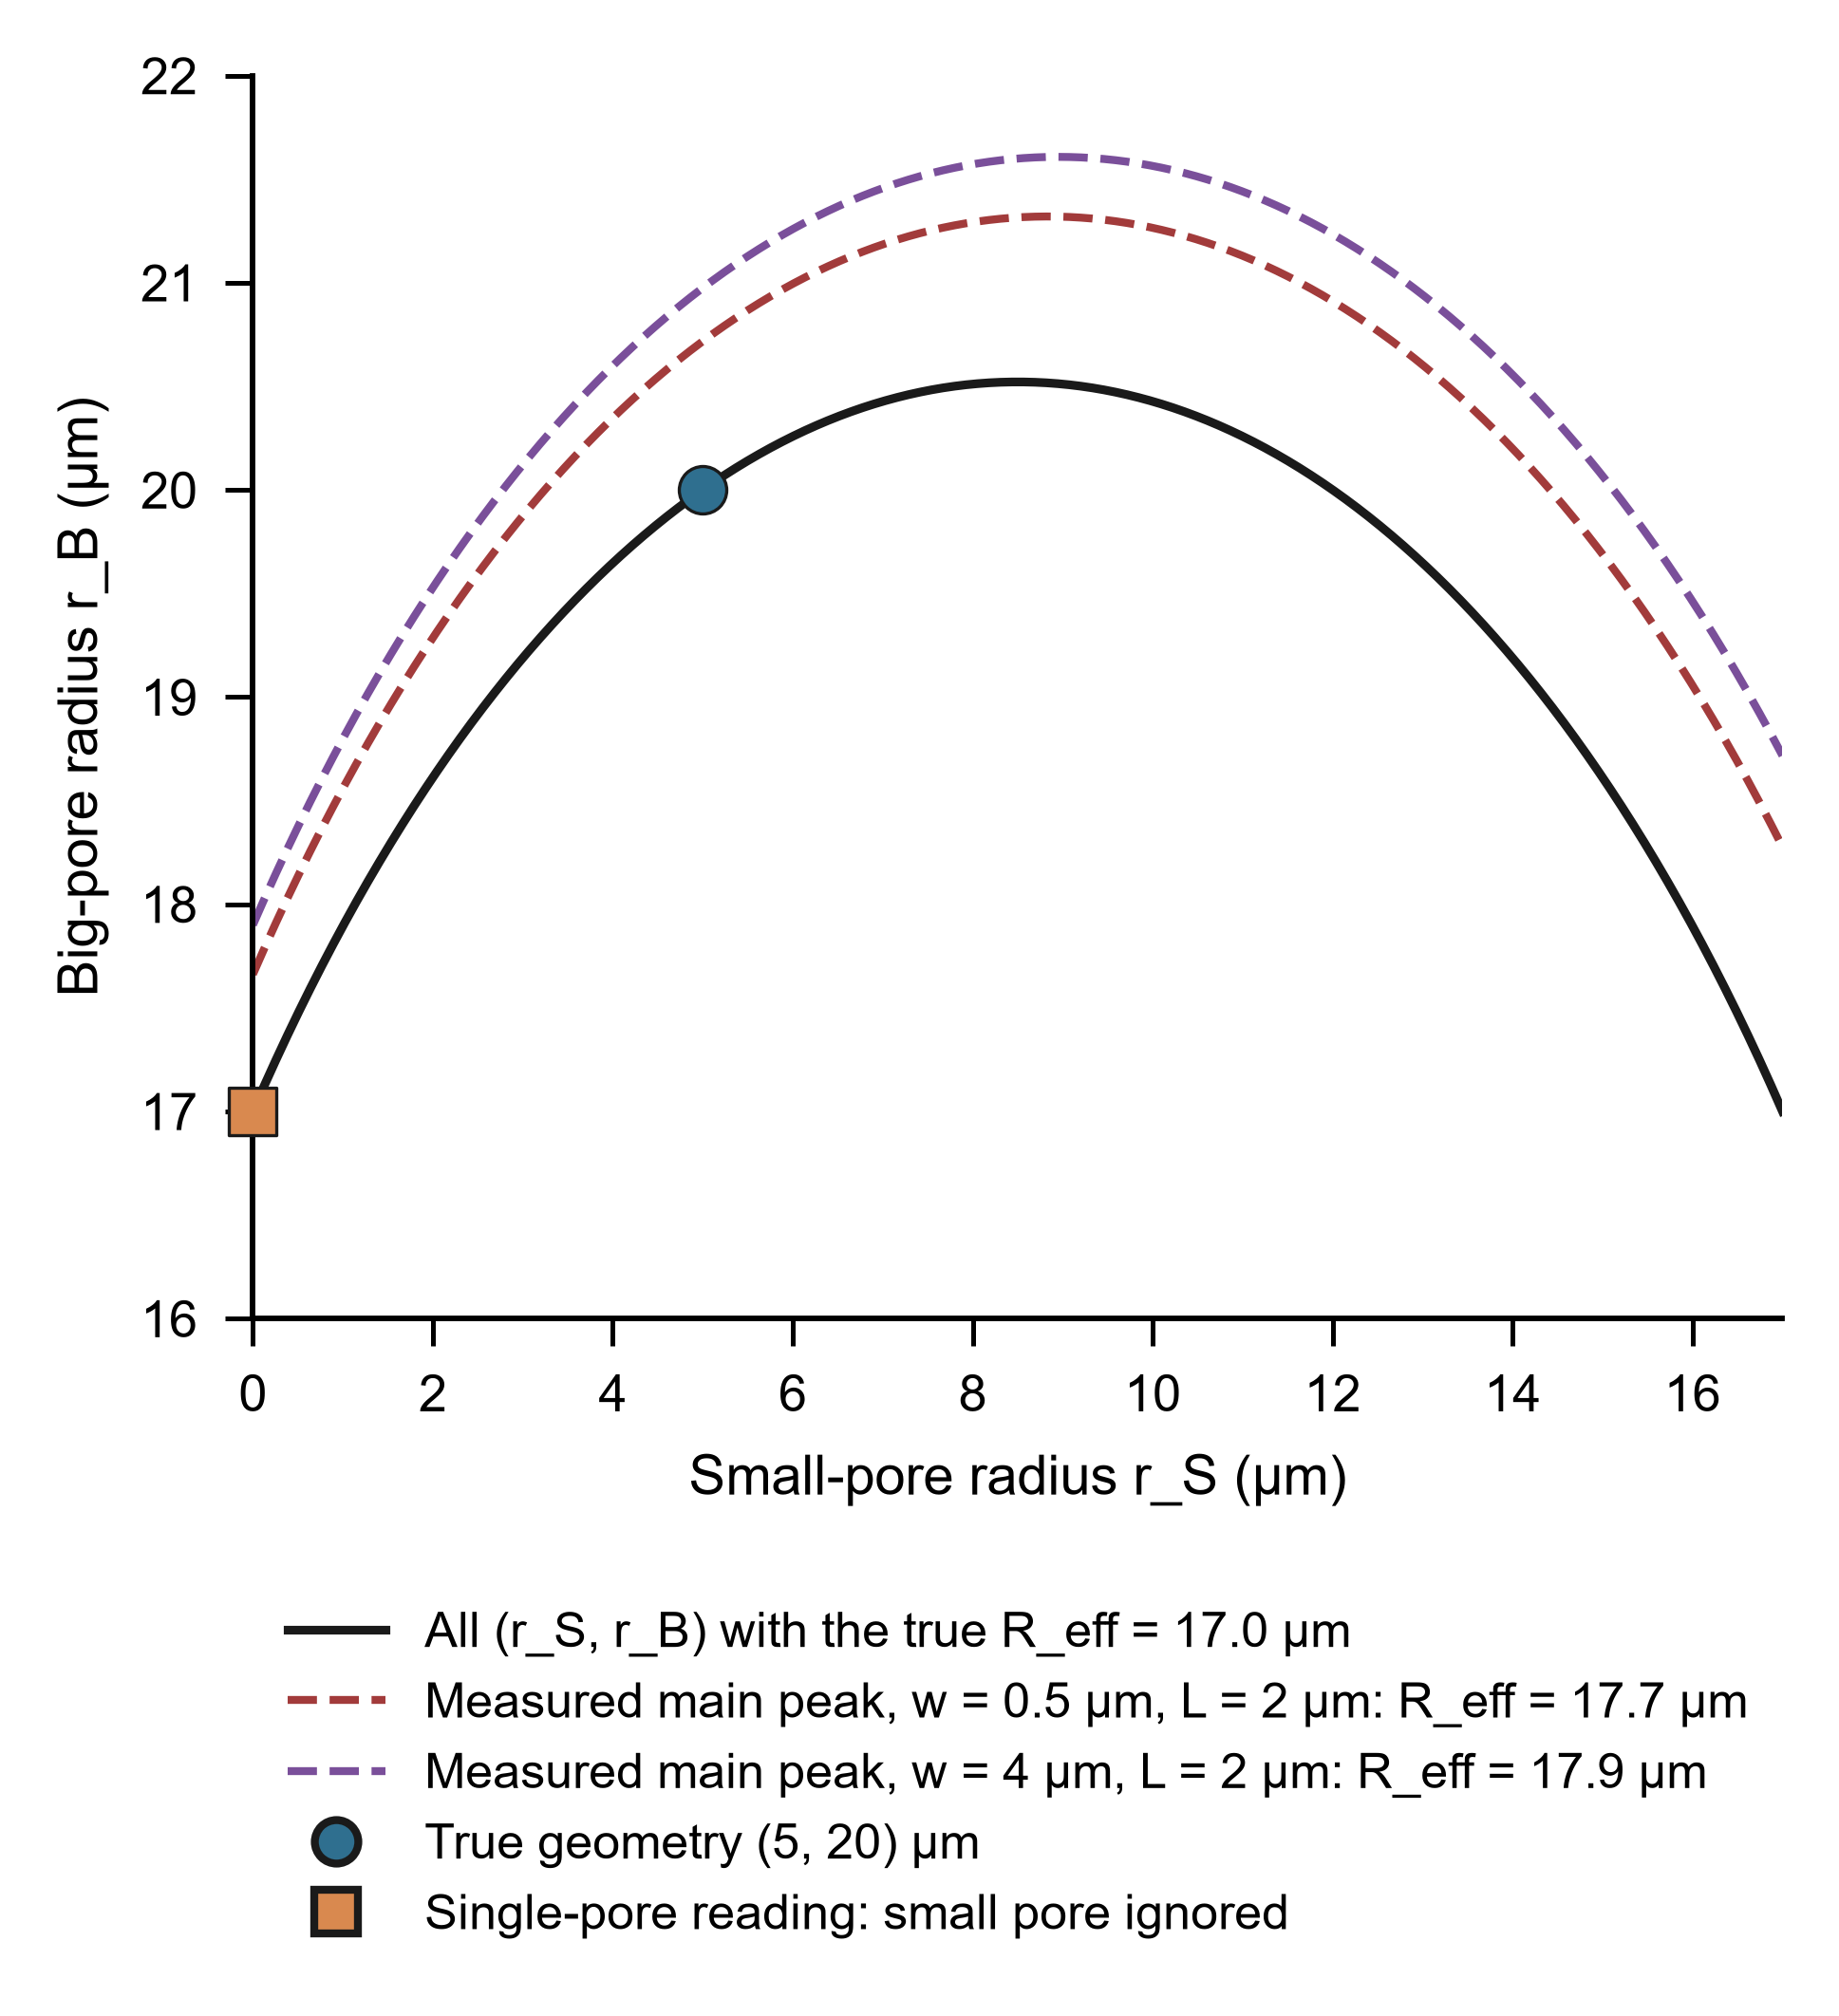
\includegraphics[width=0.55\textwidth]{fig5_nonuniqueness_fast_exchange.png}
\caption{区 III 的非唯一性：与主峰一致的全部 $(r_S,r_B)$ 组合。}
\label{fig:nonunique}
\end{figure}

\subsection{信噪比的限制}
同一衰减在 SNR 100 下重新反演（表~\ref{tab:snr}，图~\ref{fig:snr}）：区 III 的小峰全部消失；区 I、II 小峰虽保留，但分数降至 0.9–1.8\%、
$T_{2\mathrm{lm}}$ 被正则化拉到 58–143~ms，路线 D 也只能给出 $r_S\approx1.9$–$2.4$~\si{\micro m}。
即“小孔被忽略”有两层原因：物理上快交换把小孔信号并入主峰（$A_f\propto\Peff^{-2}$），测量上低 SNR 的正则化抹掉了剩余的小峰。

\begin{figure}[H]
\centering
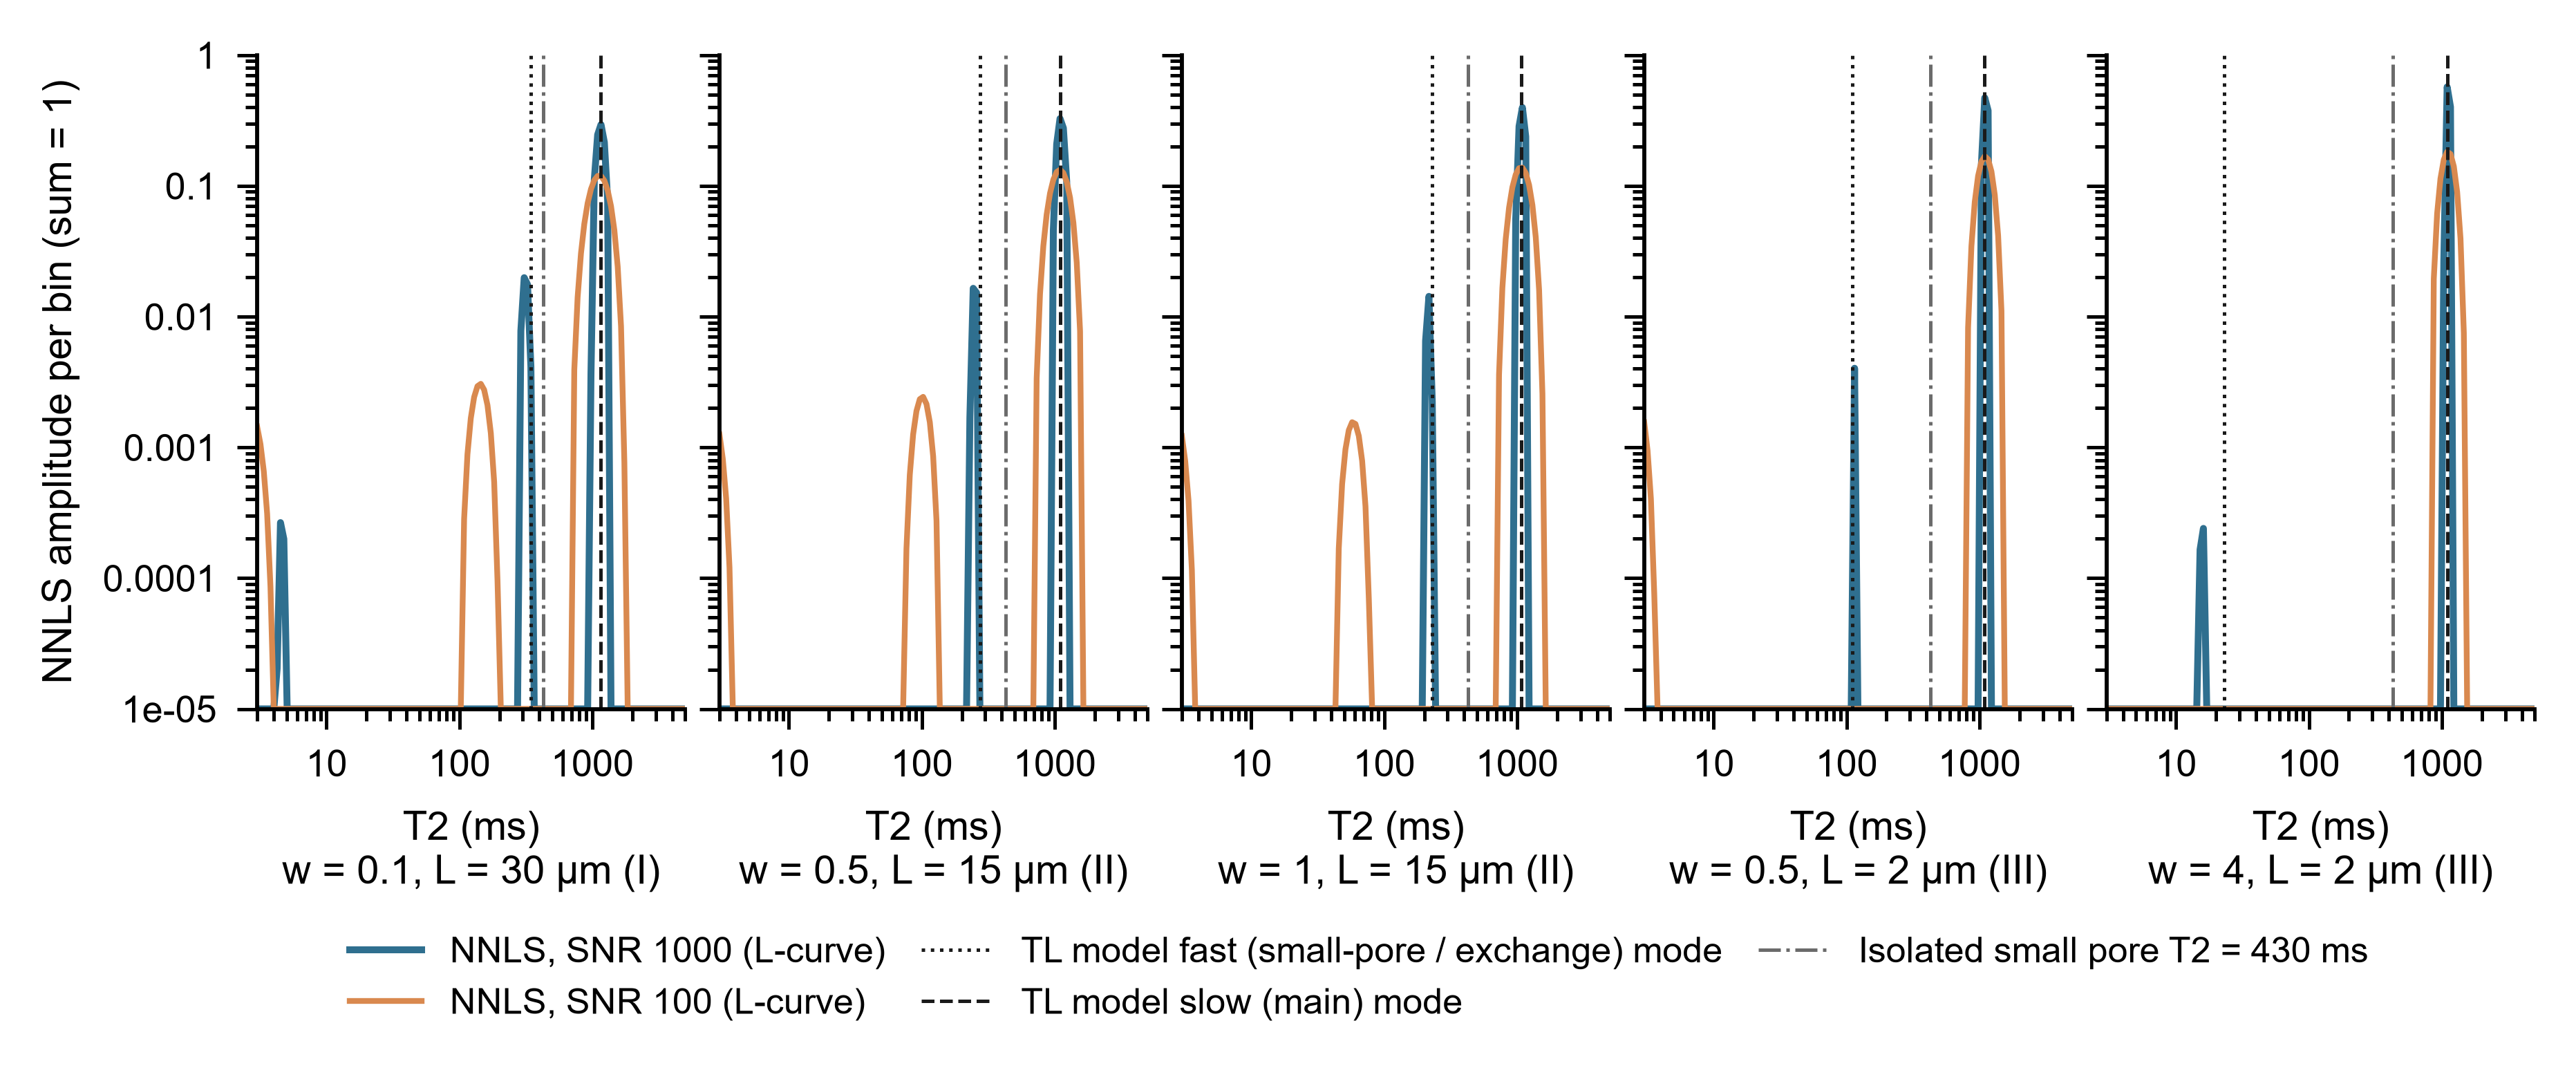
\includegraphics[width=\textwidth]{fig4_spectra_snr.png}
\caption{代表算例的 NNLS 谱（对数纵轴）：SNR 1000 与 SNR 100；竖线为 TL 模型的快、慢模态与孤立小孔 $T_2$。}
\label{fig:snr}
\end{figure}

\section{反算流程}
\begin{enumerate}[leftmargin=2em]
\item NNLS（L-curve）反演，识别高于噪声底的峰（本例 SNR 1000 时底噪约 0.2\%；$T_2<4\,T_E$ 的分量不作孔隙解释）。
\item \textbf{只有一个峰：}报告 $R_{\mathrm{eff}}$（式 \eqref{eq:reff}），并说明它是快交换下全部连通孔的 $S/V$ 等效尺寸；小孔可能被隐藏，需外部约束。
\item \textbf{两个峰：}先用路线 B 得到 $r_S$、$r_B$ 初值；若有喉道信息，计算 $\Peff$ 与 $\eta$ 判断分区：
区 I 可直接采用路线 B（或 A+汇修正），区 II 必须用路线 D。
\item \textbf{自洽检验：}以反算的 $(r_S,r_B)$ 与喉道参数正演 TL 模型，确认 $\Peff$ 落在所用路线的适用区，并与实测谱比较。
\item \textbf{SNR 要求：}次峰分数需远高于底噪；SNR 100 时即使在区 I 也会严重低估小孔。
\end{enumerate}

\section{适用边界}
\begin{itemize}[leftmargin=2em]
\item 二维模型；三维圆柱喉道的截面积 $\propto r_t^2$，汇与交换都比二维狭缝弱，$\Psi$ 的几何因子需相应修改。
\item 孔内快扩散（$\kappa\le0.05$）与喉道横向快平衡（$h^2/D\ll T_2$）；$w=\SI{4}{\micro m}$ 时喉口不再远小于小孔，喉道本身成为一个与小孔 $T_2$ 相近的“孔”（$h/\rho_2=\SI{400}{ms}$）。
\item 准静态约化在 $\lambda\ll R_t$ 时成立；宽喉道（$R_t$ 小）应使用精确特征方程 \eqref{eq:char}。
\item 分区阈值 $\eta=0.8$、$0.1$ 与 $p_S=0.0588$ 有关；小孔占比不同则普适曲线需重算。
\item 扩散耦合的思想与 \citet{Ramakrishnan1999}、\citet{AnandHirasaki2007} 的微–宏孔耦合分析一致；本文的 $\Peff$ 为本几何下的具体形式。
\end{itemize}

\begin{thebibliography}{13}
\setlength{\itemsep}{2pt}

\bibitem[Anand \& Hirasaki(2007)]{AnandHirasaki2007}
Anand, V., \& Hirasaki, G. J. (2007). Diffusional coupling between micro and macroporosity for NMR relaxation in sandstones and grainstones.
\emph{Petrophysics}, \emph{48}(4), 289--307.

\bibitem[Brownstein \& Tarr(1979)]{BrownsteinTarr1979}
Brownstein, K. R., \& Tarr, C. E. (1979). Importance of classical diffusion in NMR studies of water in biological cells.
\emph{Physical Review A}, \emph{19}(6), 2446--2453. \url{https://doi.org/10.1103/PhysRevA.19.2446}

\bibitem[Carslaw \& Jaeger(1959)]{CarslawJaeger1959}
Carslaw, H. S., \& Jaeger, J. C. (1959). \emph{Conduction of heat in solids} (2nd ed.). Oxford, UK: Clarendon Press.

\bibitem[Fleury \& Soualem(2009)]{FleurySoualem2009}
Fleury, M., \& Soualem, J. (2009). Quantitative analysis of diffusional pore coupling from T2-store-T2 NMR experiments.
\emph{Journal of Colloid and Interface Science}, \emph{336}(1), 250--259.（卷期页码请核对原文）

\bibitem[Grebenkov(2007)]{Grebenkov2007}
Grebenkov, D. S. (2007). NMR survey of reflected Brownian motion. \emph{Reviews of Modern Physics}, \emph{79}(3), 1077--1137.
\url{https://doi.org/10.1103/RevModPhys.79.1077}

\bibitem[Hansen(1992)]{Hansen1992}
Hansen, P. C. (1992). Analysis of discrete ill-posed problems by means of the L-curve. \emph{SIAM Review}, \emph{34}(4), 561--580.
\url{https://doi.org/10.1137/1034115}

\bibitem[Lawson \& Hanson(1974)]{LawsonHanson1974}
Lawson, C. L., \& Hanson, R. J. (1974). \emph{Solving least squares problems}. Englewood Cliffs, NJ: Prentice-Hall.

\bibitem[McDonald et~al.(2005)]{McDonald2005}
McDonald, P. J., Korb, J.-P., Mitchell, J., \& Monteilhet, L. (2005). Surface relaxation and chemical exchange in hydrating cement pastes:
A two-dimensional NMR relaxation study. \emph{Physical Review E}, \emph{72}(1), 011409. \url{https://doi.org/10.1103/PhysRevE.72.011409}

\bibitem[Ramakrishnan et~al.(1999)]{Ramakrishnan1999}
Ramakrishnan, T. S., Schwartz, L. M., Fordham, E. J., Kenyon, W. E., \& Wilkinson, D. J. (1999). Forward models for nuclear magnetic resonance
in carbonate rocks. \emph{The Log Analyst}, \emph{40}(4), 260--270.

\bibitem[Torrey(1956)]{Torrey1956}
Torrey, H. C. (1956). Bloch equations with diffusion terms. \emph{Physical Review}, \emph{104}(3), 563--565.
\url{https://doi.org/10.1103/PhysRev.104.563}

\bibitem[Zhou \& Zhang(2025)]{Zhou2025}
Zhou, \& Zhang (2025). How does pore structure affect the NMR relaxation in unsaturated porous media.
\emph{Water Resources Research}.（作者全名、卷期与 DOI 请按原文核对；$D$、$\TB$、$\rho_2$ 的参数来源。）

\bibitem[Zimmerman \& Brittin(1957)]{ZimmermanBrittin1957}
Zimmerman, J. R., \& Brittin, W. E. (1957). Nuclear magnetic resonance studies in multiple phase systems: Lifetime of a water molecule
in an adsorbing phase on silica gel. \emph{The Journal of Physical Chemistry}, \emph{61}(10), 1328--1333. \url{https://doi.org/10.1021/j150556a015}
\end{thebibliography}

\end{document}
